\section{Simulation Framework}
\label{sec:SimFramework}

\CM~is a robust object-oriented programming framework featuring meticulously crafted interfaces to facilitate extensible implementations. 
This framework seamlessly couples various model components while ensuring swift solutions through efficient utilization of computational resources via software parallelization using MPI and adaptive time increments.
In this section, we delve into the pivotal elements of \CM~, the framework tailored for conducting cardiac biomechanics (CB) simulations. 
This framework is intricately connected to two external libraries: the VTK library, employed for efficient data export, and the PETSc library, used for matrix vector operations and to solve the dynamic linear and non-linear equation systems. 
Programmed in C++, \CM~ adopts a comprehensive object-oriented programming structure, emphasizing its role as a multiscale electromechanical simulation framework.
It uses the method of finite elements, to solve the equilibrium of forces within the simulation domain.
The fundamental class structure of \CM~is shown in \autoref{fig:UML} and consists of the following components:
\paragraph{CBCardioMechanics} presents a user-friendly command line interface, proficient in parsing user input and initiating core components based on the provided instructions. 
Configuration files, adhering to the XML format, serve as conduits for parameters that configure the Model/Mesh, Solver, Exporter, Materials, and all SolverPlugins. 
Notably, all parameters are subject to override via the command line, facilitating swift testing of various configurations, such as adjusting time steps. 
Additionally, users have the flexibility to select different levels of verbosity for logging data.

\paragraph{CBModel} manages all data encompassing geometric information, undergoing population during mesh loading courtesy of CBModelLoader. 
Its primary role lies in conveying geometric details to the solver. 
Additionally, it plays a pivotal role in exporting simulation data to \nameref{subsubsec:VTK} files. 
Consequently, it undergoes updates with the most recent node positions and is enriched with supplementary information, including active stress, relative fiber length, and the Cauchy deformation tensor. 
This augmented dataset is then handed over to CBModelExporter.

\paragraph{CBSolver} tackles a nonlinear problem within each time step, leveraging PETSc's SNESSolve function to address nonlinear equation systems. 
It incorporates time integration in one of its specialized derived classes, namely CBSolverStatic and CBSolverNewmarkBeta. 
Responsible for overarching tasks such as step size computation, invocation of solver plugins, and mesh exporting, the CBSolver's Run() function orchestrates these operations. 
Featuring distinct data structures formatted for efficient computation, including parallel PETSc matrices and vectors, CBSolver necessitates conversion to a CBModel object before exporting. 
Instead of directly computing new node coordinates, the SolverStep() function calculates displacements in each time step, subsequently adding them to node positions from the preceding time step.

\paragraph{CBSolverPlugin} serves as a comprehensive interface to extend the solver's capabilities. 
The class defines essential functions such as Init(), Apply(), StepBack(), and Export(). 
These functions are invoked before commencing the simulation, during each solver step for updating internal information, after each unsuccessful solver step for reverting to the previous state, and after each successful solver step, complying with an export time condition, for writing information into the model and/or a text file. 
SolverPlugins wield influence over the subsequent time step through return codes like CBStatus::SUCCESS (indicating permission for the solver to advance to the next time step), CBStatus::FAILED (suggesting a reduction in time step due to plugin dissatisfaction with results), or CBStatus::REPEAT (prompting the solver to recompute the current time step, enabling plugins to iterate multiple times).

\paragraph{CBElement} The element structure comprises two distinct types: CBElementSolid and CBElementSurface. 
CBElementSolid is equipped with functions that populate the stiffness matrix with node derivative entries in a PETSc-compatible format. 
These functions are implicitly invoked by PETSc's SNESSolve() function, which employs the solver's NodalForcesHelperFunction() to call each solid element's CalcNodalForces(). 
This calculation determines the element's contribution to the system matrix, necessitated by the intricate structure dictated by PETSc's SNESSolve(). 
Unfortunately, this core functionality of the solver had to be implemented in a somewhat convoluted manner due to these constraints.
Each CBElementSolid is self-aware, maintaining knowledge of its current and initial node positions, fiber directions, material model, and tension model. 
This information is instrumental in computing its deformation tensor and determining the resulting contribution to the global energy derivatives. 
Each solid element is associated with a CBConstitutiveModel for passive stress computation and a CBTensionModel for active stress computation during its CalcNodalForces() operation.
In contrast, CBElementSurface is designed to handle surface forces application, volume computation, and identification of contact partners for the contact handling algorithm.

\paragraph{CBElementAdapter} serves as a central hub, holding pointers to critical global and element-specific components within \CM~for the sake of efficiency. 
Examples include pointers to the solver, constitutive model, time-stepping object, and other essential elements. 
The primary purpose is twofold: firstly, to grant each element read access to information that is technically not available within the element, such as global variables. 
To minimize memory consumption, node positions are stored only once in memory, facilitated by the solver's solution vector, with CBElementAdapter providing the location in memory.
Secondly, this global object enables elements to directly contribute to mass and stiffness matrices within the solver's data objects, fostering seamless integration of element-specific computations. 
This approach optimizes both memory usage and computational efficiency throughout \CM.

\paragraph{CBConstitutiveModel} provides the functions CalcEnergy() and CalcPK2Stress(), empowering each solid element to compute its deformation energy based on a provided deformation tensor, considering the passive material properties. 

\paragraph{CBTensionModel} offers functions for computing active energy contributions arising from contracting muscle fibers, utilizing a given deformation tensor. 
Specifically, CalcActiveTension() calculates the tension in the fiber direction, while CalcActiveStressTensor() determines the contribution to the PK2 stress. 
The structure closely aligns with CBConstitutiveModel, reflecting a consistent approach to handling active stress computations within the framework.\\

The object-oriented nature of the codebase allows for the seamless interchangeability and extension of specialized modules. 
For example, specializations of the CBElement class include CBElementSolidT4 and CBElementSolidT10. 
Similarly, specializations of the CBConstitutiveModel class encompass CBConstitutiveModelGuccione and CBConstitutiveModelMooneyRivlin. 
Despite their unique functionalities, all these specializations adhere to the same interface functions, ensuring compatibility and ease of integration within the system.

\begin{figure}[h!t]
    \centering
    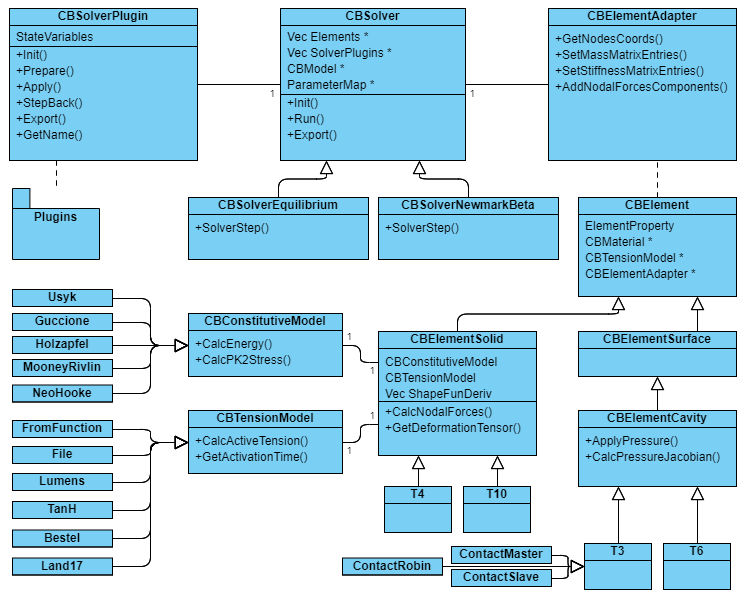
\includegraphics[width=1\linewidth]{Graphics/CardioMechanics_ClassDiagram.png}
    \caption{Fundamental structure of the simulation framework \CM.}
    \label{fig:UML}
\end{figure}

\subsection{Mesh}
\label{settings:Mesh}

The tag \verb+Mesh+, contains all parameters for the configuration of the model/geometry.
The mesh has to be provided in the TetGen format.
See \nameref{nodeFile}, \nameref{eleFile}, \nameref{surFile}, and \nameref{basesFile} for details about this format.
Only linear (\verb+T4+) and quadratic tetrahedral (\verb+T10+) elements are supported as volume elements.
During the initialization process, you can choose the method of domain decomposition.
This can either be done by node index (\verb+None+) or by principal component analysis (\verb+PCA+) of initial node coordinates.
A third variant is available using the \verb|Solver.DomainDecomposition| tag, which uses information from the stiffness matrix to minimize communication cost (becomes more relevant in HPC applications).

Surfaces and surface types for boundary condition applications have to be defined using the \verb|Surface| tag.
Only linear (\verb|T3|) and quadratic (\verb|T6|) triangular elements are supported.
However, most plugins supplying traction forces are only implemented for linear triangles.
See the code example below for available options.

The tag \verb|Transform| can be used to transform linear to quadratic elements on the fly.
This is only recommended for testing purposes.

Finally, a \nameref{LATFile} can be defined, if you want to run mechanical simulations with precalculated electrophysiological activations, \eg from solutions to the eikonal equation.

\begin{lstlisting}[language=XML,caption=.xml settings for mesh initialization]
<Mesh>
    <Type>		T4/T10 		</Type>
    <Format>	Tetgen 		</Format>
    <Sorting>	None/PCA	</Sorting>
    <Tetgen>
        <Unit>  1e-3			</Unit>
        <Nodes> filename.node	</Nodes>
        <Elements>  filename.ele 	</Elements>
        <Surfaces>  filename.sur 	</Surfaces>
        <Bases> filename.bases 	</Bases>
        <DetermineNeighbors>    true/false		</DetermineNeighbors>
        <EnforceOrthonormalBases>	true/false		</EnforceOrthonormalBases>
    </Tetgen>

     <!-- Define a surface with material number XXX and one of the following surface types: 
     CAVITY - for closed surfaces used in the circulatory system
     T3, T6 - arbitrary surfaces
     CONTACT_ROBIN - for a generalized Robin boundary condition
     CONTACT_MASTER/CONTACT_SLAVE - for the contact handling plugin based on Fritz et al. 2013 -->
    <Surfaces>
        <Surface_XXX> surfaceType </Surface_XXX>
    </Surfaces>

    <!-- Transform linear elements to quadratic elements on the fly -->
    <Transform>
    	<T4toT10> 	false </T4toT10>
    	<T3toT6> 	false </T3toT6>
    </Transform>

    <!-- Define a filename with local activation times (LAT) -->
    <LAT>
        <FilePath> filename.txt </FilePath>
    </LAT>
</Mesh>
\end{lstlisting}

\subsection{Materials}
\label{settings:Material}

The tag \verb|Materials| contains all parameters for the definition of material properties.
Using the tag \verb|Global.Damping|, the user should define the parameters for Rayleigh damping of the form $\vec C = \alpha \vec M + \beta \vec K$.
Furthermore, the user can set default material parameters using the tag \verb|Mat_Default|.
The parameters defined under this scope are valid for all materials unless specific material definitions are available.
You can define different constitutive models and tension models for each individual material if you wish to do so.

In the example below, default parameters for the density and the Usyk constitutive law are set.
If the tag \verb|IgnoreCorruptElements| is set to \verb|true|, elements with $\det(\vec F) \leq 0$ are ignored and do not contribute to the stiffness matrix.
For obvious reasons, this setting is not recommended for use.
Additionally, a material defined by number 30 is defined.
It uses the Usyk constitutive law with additional scaling applied to the default parameters as well as the Land17 tension model.
\verb|TensionMax| is set to 1000, since tension in the Land model is in \si{kPa} and we need to scale it to \si{Pa}.

In the following sections, the configurations for all available constitutive laws and tension models are discussed.

\begin{lstlisting}[language=XML,caption=.xml settings for material definitions]
<Materials>
    <Global>
        <Damping>
            <Rayleigh>
                <Alpha> 500 </Alpha>
                <Beta> 0.005 </Beta>
            </Rayleigh>
        </Damping>
    </Global>

    <Mat_Default>
        <IgnoreCorruptElements> true/false </IgnoreCorruptElements>
        <Density> 1082 </Density>
        <Usyk>
            <a>880</a> <!-- Pa -->
            <bff>8</bff>
            <bss>6</bss>
            <bnn>3</bnn>
            <bfs>12</bfs>
            <bfn>3</bfn>
            <bns>3</bns>
            <k>650e3</k> <!-- Pa -->
        </Usyk>
    </Mat_Default>
    
    <Mat_30> 
        <Type>Usyk</Type>
        <Usyk>
            <aScale>0.07</aScale>
            <bScale>3.55</bScale>
        </Usyk>

        <TensionMax>1e3</TensionMax>
        <TensionModel>Land17</TensionModel>
        <Land17>
            <CalciumTransientType>Elphy</CalciumTransientType>
            <rateDependancy>ON</rateDependancy>
            <cycleLength>0.8</cycleLength>
            <beta0>0.7</beta0>
            <beta1>-1.2</beta1>
            <Ca50>0.805</Ca50>
            <Tref>440</Tref>
        </Land17>
    </Mat_30>
    
    ...
</Materials>
\end{lstlisting}

\subsubsection{Constitutive Models}

The material constitutive laws that are used in the balance of momentum equation relate the strain of the body with its stress.
However, in cardiac mechanics, the focus is on elastic materials or in particular hyperelastic ones, i.e. the behaviour of the material is path-independent.
As a consequence, we can define a stored strain energy density function $\Psi$ to express the first Piola-Kirchhoff stress tensor as 
\begin{equation}
    \vec P (\vec F (\vec X), \vec X) = \pdv{\Psi (\vec F (\vec X), \vec X)}{\vec F} \,,
\end{equation}
or in terms of the symmetric second Piola-Kirchhoff stress tensor 
\begin{equation}
    \vec S (\vec C (\vec X), \vec X) = 2 \pdv{\Psi(\vec C (\vec X), \vec X)}{\vec C} = \pdv{\Psi(\vec E (\vec X), \vec X)}{\vec E} \,.
\end{equation}
If the relationship between $\Psi$ and $\vec C$ is independent of the material axes, $\Psi$ can be expressed as a function of the invariants of $\vec C$ as 
\begin{equation}
    \Psi(\vec C (\vec X), \vec X) = \Psi(\I{C},\II{C},\III{C}, \vec X) \,,
\end{equation}
where the invariants are defined as 
\begin{align}
    \I{C} &= \tr\vec C = \vec C : \mathds{1} \\
    \II{C} &= \frac{1}{2} \left( (\tr \vec C)^2 - \tr \vec C^2 \right) \\
    \III{C} &= \det\vec C = J^2 \,.
\end{align}
It can also be convenient to consider isochoric invariants, replacing $\vec C$ with $\vec{\bar{C}} = J^{-2/3} \vec C = \III{C}^{-1/3} \vec C$.
Furthermore, pseudo invariants can be introduced that describe the squared stretch along microstructural directions in anisotropic materials such as the myocardium:
\begin{equation}
    \mathrm{I}_{ab} = \vec C : \text{sym}(\vec e_a \otimes \vec e_b) \qc a,b \in \{f,s,n\} \,,
\end{equation}
where $\text{sym}(\vec A) = \frac{1}{2} (\vec A + \vec A^\mathrm{T})$ is the symmetric transformation.
Near incompressibility can be achieved in hyperelastic materials by adding a volumetric energy component $U(J)$ to the distortional component $\Psi (\vec{\bar{C}} )$:
\begin{equation}
    \Psi(\vec C) = \Psi (\vec{\bar{C}} ) + U(J) \,,
\end{equation}
and 
\begin{equation}
    \vec S = 2 \pdv{\Psi (\vec{\bar{C}} )}{\vec C} + 2 \dv{U(J)}{J}\pdv{J}{\vec C}  \,.
\end{equation}
In the following, the constitutive models that are implemented in \CM~are described with their respective parameters.

\paragraph{Guccione}
The incompressible strain energy density by Guccione et al.~\cite{guccione95} is given by
\begin{align}
    \Psi^{(\mathrm{G})} (\vec C) &= \frac{\kappa}{2} (J-1)^2 + \frac{\mu}{2}(\exp(Q) -1) \,, \nonumber\\
    Q &= b_\text{f} E_\text{ff}^2 + 
    b_\text{t} (E_\text{ss}^2 + E_\text{nn}^2 + E_\text{ns}^2 + E_\text{sn}^2) +
    b_\text{fs} (E_\text{fs}^2 + E_\text{sf}^2 + E_\text{fn}^2 + E_\text{nf}^2) \,,\label{eq:guccione}
\end{align}
where $E_\text{ij} = \vec E \vec i_0 \cdot \vec j_0$ for $i,j \in \{f,s,n\}$ are the entries of the Green-Lagrange strain tensor ${\vec E = \frac{1}{2}(\vec C - \mathds{1})}$.
The 2nd Piola-Kirchhoff stress is given by
\begin{equation}
    \vec S = 
    \mu \exp(Q) (b \odot E)_{ij} + \kappa (J-1) J \vec C^{-1} \qq{with} \vec b = 
    \mqty( b_\text{f} &  b_\text{fs} &  b_\text{fs} \\ 
           b_\text{fs} &  b_\text{t} &  b_\text{t} \\ 
           b_\text{fs} &  b_\text{t} &  b_\text{t}) \,,
\end{equation}
where $(A \odot B)_{ij} = (A)_{ij}(B)_{ij}$ is the Hadamard or Schur product of the matrices $\vec A$ and $\vec B$.

\begin{lstlisting}[language=XML,caption=.xml settings for Guccione material]
    <Type>Guccione</Type>
    <Guccione>
        <C>FLOAT</C> <!-- shear modulus [Pa] -->
        <bf>FLOAT</bf>
        <bt>FLOAT</bt>
        <bfs>FLOAT</bfs>
        <K>FLOAT</K> <!-- bulk modulus [Pa] -->
        <aScale>FLOAT</aScale> <!-- optional scaling for C (default 1) -->
        <bScale>FLOAT</bScale> <!-- optional scaling for b (default 1) -->
    </Guccione>
\end{lstlisting}

\paragraph{MooneyRivlin}
The Mooney-Rivlin material is a commonly used isotropic material law.
The following more general form is implemented in \CM:
\begin{equation}
    \Psi^{(\mathrm{MR})} (\I{C},\II{C}) = 
    \sum_{i=0}^2 \sum_{j=0}^2 \Bar{c}_{ij} (\I{C} - 3)^i (\II{C} - 3)^j \qq{with} \Bar{c}_{00} = 0 \,,
\end{equation}
using a penalty function expressed as $\ln{(\III{C})} = 0$ and the modified strain energy potential
\begin{equation}
    \hat{\Psi} = \Psi^{(\mathrm{MR})} -(c_{10} + 2 c_{01}) \ln{(\III{C})} + \frac{1}{2}\kappa (\ln{(\III{C})})^2 \,.
\end{equation}
The 2nd Piola-Kirchhoff stress tensor is given by
\begin{align}
    \vec S =&
    2 \pdv{\hat{\Psi}}{\C} = 
    2 \pdv{\Psi^{(\mathrm{MR})}}{\C} + 2(-(c_{10} + 2 c_{01}) + \kappa \ln{(\III{C})})\C^{-1} \,,
\end{align}
where
\begin{align}
    2 \pdv{}{\C}\Psi^{(\mathrm{MR})} &= 
    2 \left( \pdv{\Psi^{(\mathrm{MR})}}{\I{C}} \pdv{\I{C}}{\C} + \pdv{\Psi^{(\mathrm{MR})}}{\II{C}} \pdv{\II{C}}{\C} \right)  \\
    &= 2 \left( \pdv{\Psi^{(\mathrm{MR})}}{\I{C}} + \I{\C}\pdv{\Psi^{(\mathrm{MR})}}{\II{C}} \right) \mathds{1} - 2 \pdv{\Psi^{(\mathrm{MR})}}{\II{C}} \C \,,
\end{align}
with
\begin{align}
    \pdv{\Psi^{(\mathrm{MR})}}{\I{C}} &= c_{10} + 2 c_{20} (\I{C} - 3) + c_{11} (\II{C} - 3) \,,\\
    \pdv{\Psi^{(\mathrm{MR})}}{\II{C}} &= c_{01} + 2 c_{02} (\II{C} - 3) + c_{11} (\I{C} - 3)\,.
\end{align}

\begin{lstlisting}[language=XML,caption=.xml settings for general Rivlin material]
    <Type>MooneyRivlin</Type>
    <MooneyRivlin>
        <C10>FLOAT</C10> <!-- [Pa] -->
        <C01>FLOAT</C01> <!-- [Pa] -->
        <C20>FLOAT</C20> <!-- default 0 -->
        <C02>FLOAT</C02> <!-- default 0 -->
        <C11>FLOAT</C11> <!-- default 0 -->
        <B>FLOAT</B> <!-- bulk modulus [Pa] -->
    </MooneyRivlin>
\end{lstlisting}

\paragraph{Holzapfel}
The incompressible Holzapfel-Odgen strain energy density~\cite{Holzapfel-2009-ID13072} can be written as a sum of isotropic and anisotropic components
\begin{align}
    \Psi^{(\mathrm{HO})} (\vec C) = 
    &\frac{a}{2b} [\exp(b (\bar{\mathrm{I}}_{\vec C} - 3)) -1 ]
    + \sum_{kl \in S} \frac{a_{kl}}{2b_{kl}} [\exp(b_{kl} (\mathrm{I}_{kl} - \delta_{kl})^2) -1 ] \nonumber \\ 
    &+ \frac{\kappa}{4} (J^2 - 1 - 2\ln{J}) \label{eq:holzapfel} \,,
\end{align}
where $\delta_{kl}$ denotes the Kronecker delta (zero unless $k=l$, in which case it is 1) and $S = \{ff, ss, fs\}$.
The anisotropic invariants $\mathrm{I}_{ff}$ and $\mathrm{I}_{ss}$ do not support compression.
Therefore, the associated strain energy density terms are zero if $\mathrm{I}_{ff},\mathrm{I}_{ss} < 1$.
The 2nd Piola-Kirchhoff stress tensor is given by
\begin{align}
    \vec S =&
    \frac{\kappa}{2} (J - \frac{1}{J}) J \vec C^{-1}
    + \frac{a}{ J^{2/3}} \exp(b (\bar{\mathrm{I}}_{\vec C} - 3)) [\mathds{1} - \frac{1}{3} \I{C} \vec C^{-1}] \nonumber \\
    &+ \sum_{kl \in S} 2 a_{kl} (\mathrm{I}_{kl} - 1) \exp(b_{kl} (\mathrm{I}_{kl} - \delta_{kl})^2) \text{sym}(\vec e_k \otimes \vec e_l) \,.
\end{align}
The terms with $kl \in S = \{ff,ss\}$ include an approximation to the Heavyside function $\chi(\mathrm{I}_{kl}) \approx \frac{1}{1+\exp{-k(\mathrm{I}_{kl}-1)}}$.
With $k = 0$, we explicitly set $\chi(\mathrm{I}_{kl}) = 1$ if $\mathrm{I}_{kl} \leq 1$, else $\chi(\mathrm{I}_{kl}) = 0$.

\begin{lstlisting}[language=XML,caption=.xml settings for Holzapfel material]
    <Type>Holzapfel</Type>
    <Holzapfel>
        <a>FLOAT</a> <!-- [Pa] -->
        <b>FLOAT</b> <!-- [Pa] -->
        <af>FLOAT</af>
        <bf>FLOAT</bf>
        <as>FLOAT</as>
        <bs>FLOAT</bs>
        <afs>FLOAT</afs>
        <bfs>FLOAT</bfs>
        <kappa>FLOAT</kappa> <!-- bulk modulus [Pa] -->
        <k>FLOAT</k> <!-- optional (default: 100) -->
    </Holzapfel>
\end{lstlisting}

\paragraph{Usyk}
The incompressible strain energy density by Usyk et al.~\cite{Usyk-2000-ID14569} is given by
\begin{align}
    \Psi^{(\mathrm{U})} (\vec C) &= \frac{\kappa}{2} (\ln{J})^2 + \frac{\mu}{2}(\exp(Q) -1) \,, \nonumber\\
    Q &= b_\text{ff} E_\text{ff}^2 + b_\text{ss} E_\text{ss}^2 + b_\text{nn} E_\text{nn}^2
         + b_\text{fs} (E_\text{fs}^2 + E_\text{sf}^2) + b_\text{fn} (E_\text{fn}^2 + E_\text{nf}^2)
         + b_\text{ns} (E_\text{ns}^2 + E_\text{sn}^2) \,, \label{eq:usyk}
\end{align}
where $E_\text{ij} = \vec E \vec i_0 \cdot \vec j_0$ for $i,j \in \{f,s,n\}$ are the entries of the Green-Lagrange strain tensor ${\vec E = \frac{1}{2}(\vec C - \mathds{1})}$.
The 2nd Piola-Kirchhoff stress is given by
\begin{equation}
    \vec S = 
    \mu \exp(Q) (b \odot E)_{ij} + \kappa \ln(J) \vec C^{-1} \qq{with} \vec b = \mqty( b_\text{ff} &  b_\text{fs} &  b_\text{fn} \\ 
    b_\text{sf} &  b_\text{ss} &  b_\text{sn} \\ 
    b_\text{nf} &  b_\text{ns} &  b_\text{nn}) \,,
\end{equation}
where $(A \odot B)_{ij} = (A)_{ij}(B)_{ij}$ is the Hadamard or Schur product of the matrices $\vec A$ and $\vec B$.
In general, the shear stress components are assumed to be of equal contribution 
\begin{equation}
    b_{ij} = b_{ji} \qfor i \neq j \,.
\end{equation}

\begin{lstlisting}[language=XML,caption=.xml settings for Usyk material]
    <Type>Usyk</Type>
    <Usyk>
        <a>FLOAT</a> <!-- shear modulus [Pa] -->
        <bff>FLOAT</bff>
        <bss>FLOAT</bss>
        <bnn>FLOAT</bnn>
        <bfs>FLOAT</bfs>
        <bfn>FLOAT</bfn>
        <bns>FLOAT</bns>
        <k>FLOAT</k> <!-- bulk modulus [Pa] -->
        <aScale>FLOAT</aScale> <!-- optional scaling for a (default 1) -->
        <bScale>FLOAT</bScale> <!-- optional scaling for b (default 1) -->
    </Usyk>
\end{lstlisting}

\paragraph{NeoHooke}
A nearly incompressible Neo-Hookean material is defined by the hyperelastic energy potential
\begin{equation}
    \Psi^{(\mathrm{NH})} (\vec C) = \frac{\mu}{2} (\tr \bar{\vec C} - 3) + \frac{\kappa}{2}(J-1)^2 \,, \label{eq:neohooke}
\end{equation}
with the shear modulus $\mu$, the bulk modulus $\kappa$, and the 2nd Piola-Kirchhoff stress
\begin{align}
    \vec S &= \mu \pdv{\tr \bar{\vec C}}{\vec C} + \kappa \dv{(J-1)^2}{J} \pdv{J}{\vec C} \nonumber \\
    &= \mu \pdv{( \III{C}^{-1/3} \vec C : \mathds{1} )}{\vec C}  + \kappa 2(J-1) \cdot \frac{1}{2} J \vec C^{-1} \nonumber \\
    &= \mu \qty[\III{C}^{-1/3} \mathds{1} - \frac{1}{3}\III{C}^{-1/3 - 1} \III{C} \vec C^{-1} (\vec C : \mathds{1}] + \kappa (J-1) J \vec C^{-1} \nonumber  \\
    &= \mu \III{C}^{-1/3} (\mathds{1} - \frac{1}{3} \I{C} \vec C^{-1}) + \kappa (J-1) J \vec C^{-1} \,,
\end{align}
where the relationship $\pdv{\III{C}}{\vec C} = J^2 \vec C^{-1}$ was used.

\begin{lstlisting}[language=XML,caption=.xml settings for NeoHooke material]
    <Type>NeoHooke</Type>
    <NeoHooke>
        <a>FLOAT</a> <!-- shear modulus [Pa] -->
        <k>FLOAT</k> <!-- bulk modulus [Pa] -->
    </NeoHooke>
\end{lstlisting}

\subsubsection{Tension Models}

\paragraph{File} provides tensions from a tension.list file. 
The actual data is outsourced and managed by a FileManager object that lives within the solver class. 
The tension between stored data gets interpolated from a CBDataFromFile* object.
You have to provide one file at location \verb|Filename| with the following content:
\begin{lstlisting}[language=Bash,caption=File structure of a tension.list file]
# TIME  # PATH to file containing the tension values for each element at TIME
\end{lstlisting}
The individual files at \verb|PATH| containing the element tension have to be binary with the following structure
\begin{lstlisting}[language=Bash,caption=File structure of individual tension files]
int32   NrElements
double  tension[0]
double  tension[1]
double  tension[...]
double  tension[n]
\end{lstlisting}

\begin{lstlisting}[language=XML,caption=.xml settings for the File tension model]
    <TensionMax> any FLOAT </TensionMax>
    <TensionModel>File</TensionModel>
    <File>
        <StartTime> 0.0 </StartTime>
        <Period> 1.0 </Period>
        <Filename> PATH </Filename>
    </File>
\end{lstlisting}

\paragraph{Lumens} is a phenomenological model based directly on measurements of length-dependent tension in myocardial cells, as detailed by Lumens et al.~\cite{lumens2009}. 
This model takes into account the current length of the muscle cell, making it noteworthy for its potential to reproduce the Starling effect. 
The initial formulation of the model is activated by a prescribed function $F_\mathrm{rise}(t)$, which computes the activation parameter $C$. 
This parameter is described as "physiologically related to intracellular calcium concentration."
In contrast to the original paper, certain constants within the formula underwent conversion to ensure consistent units representing time and space, using meters (\si{m}) and seconds (\si{s}) instead of micrometers (\si{\micro m}) and milliseconds (\si{ms}), respectively.
Additionally, for 3D simulations, $C_\mathrm{rest}$ was set to 0 to initiate the system in an equilibrium state with zero force.
The equations are
\begin{equation}
    \begin{cases}
        L_\mathrm{s} = L_\mathrm{s,ref} \exp(\epsilon_\mathrm{f}) \,, & \qq{with} \epsilon_\mathrm{f} = 1 - \lambda_\mathrm{f} \\
        F_\mathrm{rise} = 0.02 x^3 (8 - x)^2 \exp(-x) \,, & \qq{with} x = \min(8.0, \max(t/\tau_\mathrm{R})) \\
        \dv{L_\mathrm{sc}}{t} = (\frac{L_\mathrm{s} - L_\mathrm{sc}}{L_\mathrm{se,iso}} - 1) v_\mathrm{max} \,, \\
        C_\mathrm{L} = \tanh(4 \cdot \num{1e12} \cdot (L_\mathrm{sc} - L_\mathrm{sc,0})^2) \,, \\
        T_\mathrm{fun} = \tau_\mathrm{sc}(0.29 + 0.3 \cdot \num{1e6}\cdot L_\mathrm{sc}) \,, \\
        \dv{C}{t} = \frac{1}{\tau_\mathrm{R}} C_\mathrm{L} F_\mathrm{rise} + \frac{1}{\tau_\mathrm{D}} (C_\mathrm{rest} - C)/ (1 + \exp(\frac{T_\mathrm{fun} - t}{\tau_\mathrm{D}})) \,, \\
        t = t - t_\mathrm{cycle} \,, \qq{while} t > t_\mathrm{cycle} \\
        \sigma_\mathrm{fact} = C (L_\mathrm{sc} - L_\mathrm{sc,0}) \cdot \num{1e6} \cdot \frac{L_\mathrm{s} - L_\mathrm{sc}}{L_\mathrm{se,iso}} \,, & \qif L_\mathrm{sc} \geq L_\mathrm{sc,0} \,.
    \end{cases}
\end{equation}
The generated tension is given by $T_\text{a}(t) = T_\text{max} \sigma_\mathrm{fact}$.

\begin{lstlisting}[language=XML,caption=.xml settings for the Lumens tension model]
    <TensionMax> any FLOAT </TensionMax>
    <TensionModel>Lumens</TensionModel>
    <Lumens>
        <startTime> 0 </startTime> <!-- [s] -->
        <cycleLength> 0.8 </cycleLength> <!-- [s] -->
        <Filename> Path </Filename>
        <ExportIndices> ElementIndex </ExportIndices> <!-- export element data to file -->
        <Crest> 0.0 </Crest> 
        <Lsc0> 1.51 * 1e-6 </Lsc0> <!-- [m] -->
        <Lsref> 2.0 * 1e-6 </Lsref> <!-- [m] -->
        <Lseiso> 0.04 * 1e-6 </Lseiso> <!-- [m] -->
        <vmax> 7.0 * 1e-6 </vmax> <!-- [1/s] -->
        <tauD> 32.0 * 1e-3 </tauD> <!-- [s] -->
        <tauR> 48.0 * 1e-3 </tauR> <!-- [s] -->
        <tausc> 425.0 * 1e-3 </tausc> <!-- [s] -->
    </Lumens>
\end{lstlisting}

\paragraph{FromFunction} \label{tension:FromFunction} is a collection of four simple functions to calculate an active tension response.
The possibilities are \verb|Linear|, \verb|Sinus|, \verb|SinusDriver|, and \verb|DoubleHill|.
Only choose one of the function types per material.
\begin{itemize}
    \item 
    \verb|Linear| is a function increasing linearly between \verb|StartTime| and \verb|StopTime| from 0 to 1.
    \begin{equation}
        f(t) = \frac{t - t_\mathrm{start}}{t_\mathrm{stop} - t_\mathrm{start}} \,.
    \end{equation}
    The generated tension is given by $T_\text{a}(t) = T_\text{max} f(t)$.
    This function can be used for constant tension at $T_\text{max}$ by setting \verb|KeepMaxValue| to \verb|true|.

    \item 
    \verb|Sinus| is a function defining a sinus arc by using a frequency $\omega$ and phase $\phi$.
    \begin{equation}
        f(t) = 0.5 - 0.5 \cos(\omega (t - t_\mathrm{start}) + \phi) \,.
    \end{equation}
    The generated tension is given by $T_\text{a}(t) = T_\text{max} f(t)$.

    \item 
    \verb|SinusDriver| is a sinus function for easier definition of only the positive sinus arc from \verb|StartTime| to \verb|StopTime|.
    \begin{equation}
        f(t) = \sin( \frac{\pi (t - t_\mathrm{start})}{t_\mathrm{stop} - t_\mathrm{start}}) \,.
    \end{equation}
    The generated tension is given by $T_\text{a}(t) = T_\text{max} f(t)$.
    
    \item 
    \verb|DoubleHill| is a function based on the time-dependent compliance of the left ventricle.
    Active tension $T_\text{a}$ is assumed to be equal to the time course of chamber elastance $E(t)$.
    Stergiopulos et al.~\cite{Stergiopulos1996} suggested that the elastance of the left ventricle can be approximated by two Hill functions:
    \begin{align}
        &e(t) = \frac{E(t) - E_\text{min}}{E_\text{max} - E_\text{min}} = \frac{1}{k} \qty(\frac{g_\text{c}}{1 + g_\text{c}}) \qty( \frac{1}{1 + g_\text{r}}) \,, \label{eq:DH} \\
        &\qq*{with} g_\text{c} = \qty( \frac{t^\prime}{\tau_\text{c}} )^{m_\text{c}} \qc 
        g_\text{r} = \qty( \frac{t^\prime}{\tau_\text{r}} )^{m_\text{r}} \qc \nonumber \\
        &t^\prime = \mod(t - t_0, T) \qc
        k = \max(e(t)) \,. \nonumber
    \end{align}
Equation \eqref{eq:DH} is used as an active stress driver function $T_\text{a}(t) = T_\text{max} e(t)$. 
\autoref{tab:DH} shows sample parameters for atrial and ventricular tissue.

\begin{table}[htb]
    \caption{Parameters for the active stress driver function DoubleHill.}
    \label{tab:DH}
    \centering
    \vspace{10pt}
    \begin{tabular}{rll}
    \hline
    Description & Ventricles & Atria  \\
    \hline
    Contraction rate const. $m_\text{c}$		& \num{1.32}	& \num{1.99} \\
    Relaxation rate const. $m_\text{r}$		& \num{14.5}	& \num{11.2} \\
    Contraction time offset $\tau_\text{c}$	& \SI{0.215}{\second} & \SI{0.042}{\second} \\
    Relaxation time offset $\tau_\text{r}$	& \SI{0.362}{\second} & 0.138\,s \\
    Onset time $t_0$					& \SI{0.15}{\second}	& \SI{0.0}{\second} \\
    Period $T$							& \SI{0.8}{\second}	& \SI{0.8}{\second} \\
    Peak tension $T_\text{max}$ & \SI{80}{kPa} & \SI{25}{kPa} \\
    \hline
    \end{tabular}
\end{table}
\end{itemize}

\begin{lstlisting}[language=XML,caption=.xml settings for the FromFunction tension models]
    <TensionMax> any FLOAT </TensionMax>
    <TensionModel>FromFunction</TensionModel>
    <FromFunction>
        <!-- general settings valid for all functions -->
        <StartTime>0.0</StartTime>
        <StopTime>30.0</StopTime>
        <KeepMaxValue> false </KeepMaxValue>
        <!-- function specific options -->
        <Type> DoubleHill </Type>
        <DoubleHill>
            <Period> 0.8 </Period>
            <ContrTimeOffset> 0.215 </ContrTimeOffset>
            <RelaxTimeOffset> 0.362 </RelaxTimeOffset>
            <ContrRateConst> 1.32 </ContrRateConst>
            <RelaxRateConst> 14.5 </RelaxRateConst>
            <OnsetTime> 0.15 </OnsetTime>
        </DoubleHill>

        <Type> Sinus </Type>
        <Sinus>
            <Omega> 0.0 </Omega>
            <Phi> 0.0 </Phi>
        </Sinus>
    </FromFunction>
\end{lstlisting}

\paragraph{Land17} \label{tension:land17} implements the model by Land et al.~\cite{land17} with the default parameters from the original publication.
You can run this tension model in three different modes depending on your choice of the option \verb|CalciumTransientType|:
\begin{enumerate}
    \item with a predefined calcium transient for the ventricles (\verb|Coppini|) or the atria (\verb|Brixius|).
    \item a calcium transient read from an \verb|External| file (requires path to file in \verb|CalciumFile|) sampled at \SI{1}{ms} intervals.
    \item coupled to an electrophysiology solver using the option \verb|Elphy|. Currently this is only supported with \ACC, which can be used within \CM~as a plugin (refer to \nameref{plugin:acCELLerate}).
\end{enumerate}
By setting the option \verb|rateDependancy| to \verb|OFF|, stretch rate is set to $\dv{\lambda}{t} = 0$ at all times.
Internally, the model requires the same units as in the publication.
If you are unsure, refer to \cite{land17}.

\begin{lstlisting}[language=XML,caption=.xml settings for the Land17 tension model]
    <TensionMax>1000</TensionMax>
    <TensionModel>Land17</TensionModel>
    <Land17>
        <startTime> 0 </startTime> <!-- [s] -->
        <cycleLength> 1.0 </cycleLength> <!-- [s] -->
        <kff> 1.0 </kff>
        <kss> 0 </kss>
        <knn> 0 </knn>
        <ksn> 0 </ksn>
        <Filename> Path </Filename>
        <ExportIndices> ElementIndex </ExportIndices> <!-- export element data to file -->
        <rateDependancy> ON </rateDependancy> <!-- ON or OFF -->
        <CalciumTransientType> STR </CalciumTransientType> <!-- Coppini, Brixius, External (requires CalciumFile), Elphy (coupled to electrophysiology) -->
        <CalciumFile> NONE </CalciumFile>
        <TRPNn> 2.0 </TRPNn>
        <TRPNk> 0.1 </TRPNk>
        <Ca50> 0.805 </Ca50>
        <ku> 1.0 </ku>
        <nTM> 5.0 </nTM>
        <TRPN50> 0.35 </TRPN50>
        <kuw> 0.182 </kuw>
        <kws> 0.012 </kws>
        <rs> 0.25 </rs>
        <rw> 0.5 </rw>
        <gammas> 0.0085 </gammas>
        <gammaw> 0.615 </gammaw>
        <phi> 2.23 </phi>
        <Aeff> 25.0 </Aeff>
        <beta0> 2.3 </beta0>
        <beta1> -2.4 </beta1>
        <Tref> 120.0 </Tref> <!-- [kPa] -->
        <a> 2.1 </a>
        <k> 7.0 </k>
        <eta_l> 200.0 </eta_l>
        <eta_s> 20.0 </eta_s>
        <xi> 1.0 </xi>
    </Land17>
\end{lstlisting}

\paragraph{TanH} employs the phenomenological model by Niederer et al.~\cite{Niederer-2011-ID16420} to describe the temporal development of force generation:
\begin{equation}
\begin{cases}
    T_\text{a}(t,\lambda_\mathrm{f}) = T_\text{peak} \phi (\lambda) \tanh^2(\frac{t_\text{s}}{\tau_c}) \tanh^2(\frac{t_\text{dur} - t_\text{s}}{\tau_r}) & \qfor 0 < t_\text{s} < t_\text{dur} \,, \\
    \phi(\lambda_\mathrm{f}) = \max\qty{\tanh(\text{ld}(\lambda_\mathrm{f} - \lambda_0)),0}\,, & \\
    \tau_c = \tau_{c0} + \text{ld}_\text{up} (1 - \phi(\lambda_\mathrm{f}))\,, & \\
    t_\text{s} = t - t_\text{a} - t_\text{emd}\,, & \\
\end{cases} \label{eq:TanH}
\end{equation}
where $\lambda_\mathrm{f}$ is the fiber stretch ratio, $t_\text{a}$ is the time of activation, $T_\text{peak}$ is the peak tension, $t_\text{emd}$ is the electromechanical delay, $\tau_c$ is the contraction time, $\tau_r$ is the relaxation time, $\text{ld}$ is the degree of length dependence, $\text{ld}_\text{up}$ is the length dependence upstroke time, $\tau_{c0}$ is the contraction duration, and $\lambda_0$ is the minimal fiber stretch.

\begin{lstlisting}[language=XML,caption=.xml settings for the TanH tension model]
    <TensionMax>1000</TensionMax>
    <TensionModel>TanH</TensionModel>
    <TanH>
        <startTime> 0 </startTime> <!-- [s] -->
        <cycleLength> 1.0 </cycleLength> <!-- [s] -->
        <kff> 1.0 </kff>
        <kss> 0 </kss>
        <knn> 0 </knn>
        <ksn> 0 </ksn>
        <Filename> Path </Filename>
        <ExportIndices> ElementIndex </ExportIndices> <!-- export element data to file -->
        <MinFiberStretch> 0.7 </MinFiberStretch> 
        <EMD> 0.015 </EMD> <!-- [s] -->
        <PeakTension> 120 </PeakTension> <!-- [kPa] -->
        <Duration> 0.3 </Duration> <!-- [s] -->
        <ContractionTime> 0.1 </ContractionTime> <!-- [s] -->
        <DegreeOfLengthDependence> 5.0 </DegreeOfLengthDependence> 
        <LengthDependenceUpstrokeTime> 0.5 </LengthDependenceUpstrokeTime> <!-- [s] -->
        <RelaxationTime> 0.1 </RelaxationTime> <!-- [s] -->
    </TanH>
\end{lstlisting}

\paragraph{Bestel} employs the phenomenological model by Bestel et al.~\cite{Bestel}, characterized through a time-dependent stress function $T_\mathrm{a}$:
\begin{equation}
    \begin{cases}
        \dv{T_\mathrm{a}(t)}{t} = -\abs{a(t)} T_\mathrm{a}(t) + \sigma_0 \abs{a(t)}_+ \,, \\
        \abs{a(t)}_+ = \max{(a(t),0)} \,, \\
        a(t) = \alpha_\mathrm{max} f(t) + \alpha_\mathrm{min} (1 - f(t)) \,, \\
        f(t) = S^+(t - t_\mathrm{sys}) S^-(t - t_\mathrm{dias}) \,, \\
        S^\pm(\Delta t) = 0.5 (1 \pm \tanh{(\frac{\Delta t}{\gamma})}) \,,
    \end{cases} \label{eq:Bestel}
\end{equation}
where $a(t)$ is the activation function, $\sigma_0$ is the contractility, $\alpha$ is the activation rate, $\gamma$ is the steepness, $t_\mathrm{sys}$ and $t_\mathrm{dias}$ are the systolic and diastolic onset times, respectively.

\begin{lstlisting}[language=XML,caption=.xml settings for the Bestel tension model]
    <TensionMax>1</TensionMax>
    <TensionModel>Bestel</TensionModel>
    <Bestel>
        <startTime> 0 </startTime> <!-- [s] -->
        <cycleLength> 1.0 </cycleLength> <!-- [s] -->
        <kff> 1.0 </kff>
        <kss> 0 </kss>
        <knn> 0 </knn>
        <ksn> 0 </ksn>
        <Filename> Path </Filename>
        <ExportIndices> ElementIndex </ExportIndices> <!-- export element data to file -->
        <Contractility> 1e5 </Contractility> <!-- [Pa] -->
        <MaxActivationRate> 5 </MaxActivationRate>
        <MinActivationRate> -30 </MinActivationRate>
        <Steepness> 5e-3 </Steepness>
        <OnsetSystole> 0.17 </OnsetSystole> <!-- [s] -->
        <OnsetDiastole> 0.484 </OnsetDiastole> <!-- [s] -->
    </Bestel>
\end{lstlisting}

\subsection{Solver}
\label{settings:Solver}

Two different solver classes are available.
These are the \verb|Static| solver and the \verb|NewmarkBeta| solver.
The \verb|Static| solver does not require any further parameters to be set and is used to solve problems according to \autoref{eq:staticLinMom} without momentum or problems where inertial forces can be neglected.
In this case, time steps can be interpreted as loading steps instead.
Dynamic problems should be solved with the \verb|NewmarkBeta| solver, which uses the name-giving time integration method to solve the initial value problem.
It provides two parameters to control the numerical stability of the solution.
First order accuracy and unconditional stability can be achieved with $\beta = \frac{1}{4}(\gamma + \frac{1}{2})^2$ and $\gamma \geq \frac{1}{2}$.
Using $\gamma > 0.5$ enables numerical dissipation of higher frequencies.
However, it degrades the accuracy of the solver slightly.
Additionally, you can choose to use a \verb|ConsistentMassMatrix| (recommended) or a lumped mass matrix by setting the parameter to \verb|false|.
With \verb|NewmarkBeta.Type| you can choose between the \href{https://petsc.org/main/manualpages/Mat/MATSOLVERMUMPS/}{mumps} and \href{https://petsc.org/main/manualpages/Mat/MATSOLVERSUPERLU/}{superlu} solver packages to perform the factorization.

\paragraph{Adaptive Time Stepping}
Since the cardiac cycle consists of different phases that are more or less difficult to solve,
CardioMechanic's solver is equipped with an adaptive time stepping scheme.
The idea behind the time stepping is to decrease the time step by a factor of two each time a simulation step fails, and to increase it by the same factor if it succeeds. 
Increase should happen in such a way that the same points in time are hit that would be hit by the larger time steps to ensure a consistent export of data.
To prevent too many of the computationally expensive failing solver steps, the relaxation can be delayed by the following two parameters:
\begin{itemize}
    \item
    \verb|MinStep| After reduction, do at least this number of steps before trying a larger time step. 
    Should be dividable by two.
    \item 
    \verb|FastRelaxation| Allows the time step to increase by more than one level at the same time. 
    Tries always the maximum possible time step length after each export, no matter how small the time step was before.
\end{itemize}
The solver will adapt the time step size based on solver and solver plugin return codes:
\begin{itemize}
    \item \verb|CBStatus::SUCCESS|: system solved, the counter increments by one and gets subsequently checked if an increase of the step size is possible for the next solver run.
    \item \verb|CBStatus::REPEAT|: system solved, but coupling condition is not fulfilled yet.
    \item \verb|CBStatus::FAILED|: no solution was found with the current time step. Reduce time step by a factor of two.
\end{itemize}
In most cases, a \verb|TimeStep| of \SI{1}{ms} is sufficient to solve the mechanical system.
If you do not set \verb|MaxTimeStep|, \verb|TimeStep| is used instead.
Experience shows that if you observe more than two or three time step reductions during a simulation, it is highly likely that the simulation will fail sooner or later.
Typically this happens with an insufficient quality of the tetrahedral mesh.
One really bad element is all it takes to give you a lot of trouble.

\begin{lstlisting}[language=XML,caption=.xml settings for the solver class]
<Solver>
    <!-- General Settings -->
    <Precision> 1e-8 </Precision>
    <Epsilon> 1e-12 </Epsilon>
    <IgnoreMaxIt> false </IgnoreMaxIt>
    <MaxIterations> 50 </MaxIterations>
    <MaxFunEval> 1000 </MaxFunEval>
    <NonZeros> 2000 </NonZeros>
    <ExportSNESMatrix> false </ExportSNESMatrix>
    <StepUpIterations> 1000 </StepUpIterations>
    <Timing> true </Timing>
    <Formulation> TotalLagrangian </Formulation>

    <!-- Set Solver -->
    <Type> Static/NewmarkBeta </Type>
    <NewmarkBeta>
        <!-- Dissipation of higher frequencies for Gamma >= 0.5 -->
        <!-- Unconditional stability for 2*Beta >= Gamma >= 0.5 -->
        <Beta> 0.25 </Beta>
        <Gamma> 0.5 </Gamma>
        <ConsistentMassMatrix> true </ConsistentMassMatrix>
        <Type> mumps/superlu </Type>
    </NewmarkBeta>

    <!-- Timing -->
    <StartTime> 0 </StartTime>
    <StopTime> FLOAT </StopTime>
    <TimeStep> FLOAT </TimeStep>
    <MinTimeStep> 1e-9 </MinTimeStep>
    <MaxTimeStep> TimeStep </MaxTimeStep>
    <MaxInitTimeStep> MaxTimeStep </MaxInitTimeStep>
    <FastRelaxation> false </FastRelaxation>
    <MinSteps> 4 </MinSteps>
</Solver>
\end{lstlisting}

\subsection{Solver Plugins}
\label{settings:Plugins}

The solver class supports the use of plugins which have to be activated in the \verb|Solver| scope of the settings file. 
The individual plugin parameters are set in a separate \verb|Plugins| scope, which are explained in further detail in the following sections.
If you want to implement a new plugin, you should make sure and think about, which template functions defined in \href{https://github.com/KIT-IBT/CardioMechanics/blob/main/mechanics/src/CBSolverPlugins/CBSolverPlugin.h}{CBSolverPlugin.h} you need to implement.
The following is a list of the most important ones:
\begin{itemize}
    \item \verb|Init()|: called during solver initialization to initialize vectors, matrices, parameters etc.
    \item \verb|Prepare()|: called before first \verb|SolverStep()| to have access to the undeformed mesh.
    \item \verb|Apply()|: called during \verb|SolverStep()| before system is solved.
    \item \verb|StepBack()|: controls plugin behavior when a solver step failed and is repeated with a smaller time step.
    \item \verb|Export()|: primary export to VTK file called during solver export.
    \item \verb|WriteToFile()|: secondary export to arbitrary files.
    \item \verb|GetName()|: return the name of the plugin.
    \item \verb|ApplyToNodalForces()|: to calculate and add external forces to the system, \eg pressure.
    \item \verb|AnalyzeResults()|: called during \verb|SolverStep()| after system is solved. Can be used to check coupling conditions.
    \item \verb|GetStatus()|: returns status code of the plugin at the end of \verb|SolverStep()|.
\end{itemize}

\begin{lstlisting}[language=XML,caption=.xml settings for solver plugins]
<Solver>
.
.
.
    <Plugins>
        <Circulation>true/false</Circulation>
        <ContactHandling>true/false</ContactHandling>
        <LoadUnloadedState>true/false</LoadUnloadedState>
        <acCELLerate>true/false</acCELLerate>
        <ApplyPressure>true/false</ApplyPressure>
        <ApplyPressureFromFunction>true/false</ApplyPressureFromFunction>
        <ApplyPressureFromFunctionNodeExport>true/false</ApplyPressureFromFunctionNodeExport>
        <ReferenceRecovery>true/false</ReferenceRecovery>
        <RobinBoundary>true/false</RobinBoundary>
        <RobinBoundaryGeneral>true/false</RobinBoundaryGeneral>
    </Plugins>
</Solver>

<Plugins>
...
</Plugins>
\end{lstlisting}

\subsubsection{LoadUnloadedState}
The purpose of this plugin is to start a simulation using a stress and pressure free state of a geometry created from imaging.
A .node file for the unloaded and inflated state is required as input for this plugin.
They are typically acquired as a result of using the \nameref{plugin:ReferenceRecovery} plugin.

\begin{algorithm}
\caption{Algorithm of LoadUnloadedState plugin.}
\begin{algorithmic}[1]
\Procedure{LoadUnloadedState}{}
\State initialize $originalCoords\_ = nodes\_$; $unloadedCoords\_$; $inflatedCoords\_$
\State set $nodes\_ = unloadedCoords\_$
\State update shape functions
\State set $velocity\_ = 0$; $acceleration\_ = 0$
\State set $nodes\_ = inflatedCoords\_$
\State solve system once during Solver::Init()
\EndProcedure
\end{algorithmic}
\end{algorithm}

\begin{lstlisting}[language=XML,caption=.xml settings for LoadUnloadedState plugin]
    <LoadUnloadedState>
        <unloadedNodes>PATH</unloadedNodes>
        <inflatedNodes>PATH</inflatedNodes>
    </LoadUnloadedState>
\end{lstlisting}

\subsubsection{ContactHandling}
\label{plugin:ContactHandling}

This plugin models the effect of the tissue surrounding the heart according to Fritz et al.~\cite{fritz13a}, which assumes a frictionless and permanent contact between the epicardium and the pericardium using a penalty formulation.
For this purpose, the so called master ($\Gamma^\text{M}$) and slave ($\Gamma^\text{S}$) surfaces are defined as a contact interface.
$\Gamma^\text{M}$ is defined on the epicardium and $\Gamma^\text{S}$ is the inner surface of a separate volume mesh surrounding the heart.
The force acting on the master surface is given by $\vec f^\mathrm{M} = \alpha g(\vec x) \vec n$ with the penalty parameter $\alpha$, the gap function $g(\x)$, and the current surface normal vector $\vec n$.
For the slave surface, the same formulation is used except with negative sign for the contact forces $\vec f^\mathrm{S} = -\vec f^\mathrm{M}$.
The gap function $g(\vec x)$ is determined by projecting a point $\vec x^\mathrm{m} \in \Gamma^\text{M}$ onto the surface $\Gamma^\text{S}$ into the direction of the current normal direction $\vec n$.
Depending on the distance between $\vec x^\mathrm{m}$ and the projected point $\vec x^\mathrm{s} \in \Gamma^\text{S}$, the gap function reads
\begin{equation}
    g(\vec x) = 
    \begin{cases}
    \norm{\vec x^\mathrm{m} - \vec x^\mathrm{s}}^2 / 2d &\qq*{for} \norm{\vec x^\mathrm{m} - \vec x^\mathrm{s}} < d \,, \\
    \norm{\vec x^\mathrm{m} - \vec x^\mathrm{s}} - \frac{d}{2} &\qq*{for} \norm{\vec x^\mathrm{m} - \vec x^\mathrm{s}} \geq d \,, \\
    0 &\qq*{for} \norm{\vec x^\mathrm{m} - \vec x^\mathrm{s}} > d_\mathrm{max} \,,
    \end{cases}
\end{equation}
with the \verb|TransitionDistance| $d$ and the \verb|MaxDistance| $d_\mathrm{max}$ below which contact is maintained.
This adaptation to the original formulation was made to yield a smooth transition in case the surfaces $\Gamma^\text{M}$ and $\Gamma^\text{S}$ start to overlap, which results in a change of direction of $\vec n$.
$\Gamma^\text{M}$ and $\Gamma^\text{S}$ have to be defined under \verb|Mesh.Surfaces| with the respective surface type of either \verb|CONTACT_MASTER| or \verb|CONTACT_SLAVE|.
With the parameter \verb|Alpha| you can set the penalty variable in \si{Pa}.
The contact problem penalization can be ramped up during initialization to avoid large forces in the first time step.
The ramp is either linear or exponential depending on the parameter \verb|InitType| and will be carried out in $n$ discrete \verb|Steps|.
\verb|Beta| sets a multiplication factor for $\alpha$ during this phase.
The option \verb|MaxAngle| sets the maximal angle (in \si{degree}) between master and slave normals that still gets considered.
The option \verb|OneWayForce| determines if the contact force is applied in both directions (0) or if only positive (1) or negative (-1) forces are applied.
If you set \verb|SurfaceNormalDirection| as unidirectional, the forces are applied in the direction of the master surface normal.
Otherwise, master surface normal and slave surface normal are added and normalized.
The surface normal direction can be flipped during run time using \verb|FlipSurfaceNormals|.
If you find your slave surface is too far away from the heart's surface, you can use the option \verb|useContactHandlingToFitPeri| to run a short simulation to slowly bring the surface normal closer to the heart.
In such a simulation, it is recommended to fix the epicardial nodes using Dirichlet boundary conditions to avoid unwanted movement.
If you want to apply a spatially varying penalty formulation, assign the third attribute to the master surface elements in the \nameref{surFile}.
With \verb|Export| active, contact force, contact pressure, contact distance, and a binary state describing if a contact slave element was found are saved in arrays of the \nameref{subsubsec:VTK} in each time step.
Additionally, a text file with average contact distance and contact pressure is saved at \verb|ExportPath|.

\textbf{Remark: if you intent to use a combination of pericardial boundary conditions, only one plugin will export the data properly since they overwrite each others arrays. Hence, turn export only on for one of them!}

\begin{lstlisting}[language=XML,caption=.xml settings for ContactHandling plugin]
<ContactHandling>
    <Export>true/false</Export>
    <ExportPath>PATH</ExportPath>
    <MaxDistance>FLOAT</MaxDistance>
    <TransitionDistance>FLOAT</TransitionDistance>
    <MaxAngle>FLOAT</MaxAngle>
    <Alpha>FLOAT</Alpha>
    <Beta>FLOAT</Beta>
    <StartTime>FLOAT</StartTime>
    <OneWayForce>0/1/-1</OneWayForce>
    <InitType>Linear/Exponential</InitType>
    <Steps>INT</Steps>
    <useContactHandlingToFitPeri>true/false</useContactHandlingToFitPeri>
    <FlipSlaveNormals>true/false</FlipSlaveNormals>
    <SurfaceNormalDirection>unidirectional/bidirectional</SurfaceNormalDirection>
</ContactHandling>
\end{lstlisting}

\subsubsection{Circulation}
\label{plugin:Circulation}

The \verb|Circulation| plugin implements various lumped parameter circulatory system models suitable for 1-,2-, and 4-chamber heart models.
\autoref{fig:CircUML} shows the basic class structure of this plugin.
Some general settings are available for the base plugin.
Chamber volumes and pressures in each time step can be exported to \verb|IterationsFile| in CSV format.
The parameter \verb|Tolerance| decides how well 3D and 0D volumes have to match to be accepted by the solver.
Surfaces to be excluded from applying pressure to can be added to \verb|IgnoredSurfaceIndices| as a comma separated list.
\verb|PressureUnit| and \verb|VolumeUnit| define the units used for the input parameters and model outputs.
\verb|MaxIterations| is the maximum number of iterations before the plugin return \verb|CBStatus::FAILURE| to the solver.
\verb|Perturbation| defines, whether initial pressure perturbations shall be performed to determine the Jacobian at the beginning of each new time step.
\verb|SecantIterations| defines the number of iterations to be executed with the one-dimensional secant-method before perturbing the pressures (typically set to 0 in favor of the quasi Newton method described below).

\begin{lstlisting}[language=XML,caption=.xml settings for the circulation plugin]
<Circulation>
    <IgnoredSurfaceIndices> ... </IgnoredSurfaceIndices>

    <Tolerance> 1e-7 </Tolerance>
    <MaxIterations> 250 </MaxIterations>
    <MaxNonNewtonIterations> 10 </MaxNonNewtonIterations>
    <Perturbation> false </Perturbation>
    <SecantIterations> 0 </SecantIterations>
    <IterationsFile> PATH </IterationsFile>
    
    <PressureUnit> mmHg/hPa/Pa </PressureUnit>
    <VolumeUnit> ml/m3 </VolumeUnit>
    ...
</Circulation>

\end{lstlisting}

\begin{figure}
    \centering
    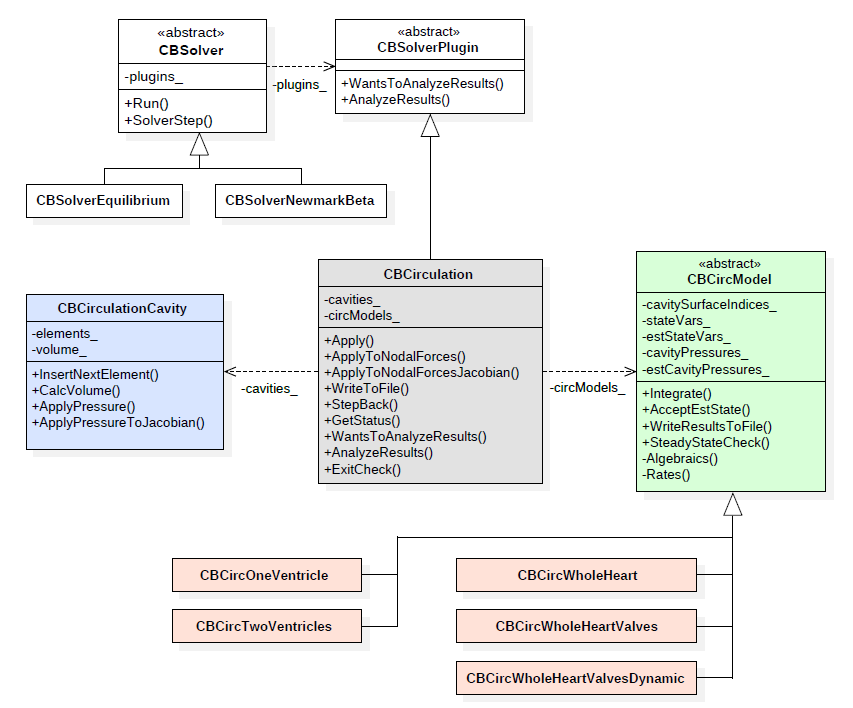
\includegraphics[width=1\linewidth]{Graphics/Circulation_UML.PNG}
    \caption{Simplified diagram of the circulation plugin class structure showing only the most important functions and variables. Created by Steffen Schuler.}
    \label{fig:CircUML}
\end{figure}

\paragraph{Coupling method} The pressure values $\p{C}$ with $\mathrm{C} \in \{\mathrm{LV,RV,LA,RA}\}$ are used as a Neumann boundary condition of the form
\begin{equation}
    \F\,\S \vec N = -\p{C}(t) J \vec F^{-\tran} \vec N \,
\end{equation}
and are computed iteratively at each time step.
In the first iteration $i=0$ of each time step $t_n$ of the mechanical system, the pressure $\p{C}$ is extrapolated from the previous 5 time steps using a 4th order Adams-Bashforth scheme:
\begin{equation} 
    \label{eq:circextrapolation}
    \p{C}^{n,0} = \p{C}^{n-1} + \Delta t_n\left(
    \frac{55}{24}\frac{\Delta \p{C}^{n-1}}{\Delta t_{n-1}}
    - \frac{59}{24}\frac{\Delta \p{C}^{n-2}}{\Delta t_{n-2}}
    + \frac{37}{24}\frac{\Delta \p{C}^{n-3}}{\Delta t_{n-3}}
    - \frac{9}{24}\frac{\Delta \p{C}^{n-4}}{\Delta t_{n-4}}
    \right)\,,
\end{equation}
with $\frac{\Delta \p{C}^k}{\Delta t_{k}} = \frac{\p{C}^k - \p{C}^{k-1}}{t_{k}- t_{k-1}}$, $k\in\mathbb{N}$.
If there are not enough pressure values available for extrapolation (\ie $n<5$), the pressure is simply increased $\p{C}^{n,0} = \p{C}^{n-1} + \SI{1}{\pascal}$.
For the sake of brevity, the four chamber pressures are now denoted $\vp{C} = (\p{LV}, \p{RV}, \p{LA}, \p{RA})^\tran$.
During consequent iterations $0 < i \leq 10$, the residual $\res{C}\colon\mathbb{R}^{4}\rightarrow\mathbb{R}^{4}$ for all chambers 
\begin{equation*}
    \res{C}(\vp{C}^{n,i})= (r_\mathrm{LV},r_\mathrm{RV},r_\mathrm{LA},r_\mathrm{RA})^\tran \,,
\end{equation*}
with $r_\mathrm{C} = \abs{\vol{C}^\mathrm{3D} - \vol{C}^\mathrm{0D}}$ is used to update $\vp{C}$ by a quasi-Newton method:
\begin{equation}
    \label{eq:quadinewton}
\vp{C}^{n,i} = \vp{C}^{n,i-1} - \vec C_i^{-1}\res{C}(\vp{C}^{n,i}) \,,
\end{equation}
where $\vec C_i$ is the compliance matrix determined by
\begin{equation*}
\vec C_i^{-1} = \vec C_{i-1}^{-1} + \left({\vartriangle} \vp{C}^{n,i}-\vec C_{i-1}^{-1}
{\vartriangle} \res{C}^{n,i}\right) \frac{{\vartriangle} (\vp{C}^{n,i})^\tran\vec C_{i-1}^{-1}}{{\vartriangle} (\vp{C}^{n,i})^\tran\vec C_{i-1}^{-1}{\vartriangle} \res{C}^{n,i}}\,,\qquad \vec C_0^{-1} = \mathds{1} \,,
\end{equation*} 
with ${\vartriangle} \vp{C}^{n,i} = \vp{C}^{n,i}-\vp{C}^{n,i-1}$, ${\vartriangle} \res{C}^{n,i} = \res{C} (\vp{C}^{n,i})-\res{C} (\vp{C}^{n,i-1})$.
Typically, this method satisfies the volume-consistency constraint 
\begin{align}
\begin{cases}
\vol{LV}^\mathrm{3D}(\d(t),\vp{C}(t)) = \vol{LV}^\mathrm{0D}(\c(t),\vp{}(t)) \qin (0,T] \,, & \\
\vol{RV}^\mathrm{3D}(\d(t),\vp{C}(t)) = \vol{RV}^\mathrm{0D}(\c(t),\vp{}(t)) \qin (0,T] \,, & \\
\vol{LA}^\mathrm{3D}(\d(t),\vp{C}(t)) = \vol{LA}^\mathrm{0D}(\c(t),\vp{}(t)) \qin (0,T] \,, & \\
\vol{RA}^\mathrm{3D}(\d(t),\vp{C}(t)) = \vol{RA}^\mathrm{0D}(\c(t),\vp{}(t)) \qin (0,T] \,, & \\
\end{cases} \label{eq:volumeConstraint}
\end{align}
with a tolerance of $\norm{\res{C}}_\infty < \varepsilon \leq \SI{1e-7}{\milli\litre}$ in 2 to 3 iterations.
During the first time steps, the quasi-Newton update might not be sufficient in which case a standard Newton method is applied and the compliance matrix is calculated using the Jacobian $\vec C = \dv{\res{C}}{\vp{C}}$ after successively perturbing one chamber at a time.

\paragraph{Coupling Damping} When the valve model is included in the circulation model, the pressures start to oscillate with a frequency corresponding to the simulation time step.
These oscillations do not decay on their own and can be explained by the effects of inertia on both sides to be coupled.
This can be avoided by using the \verb|CouplingDamping| option.
First, the coupling algorithm iterates, until the coupling criterion is fulfilled, giving the pressure estimate $\vec p^n$.
Then a pressure $\vec p^n_\mathrm{damped}$ between this pressure and the pressure $\vec p^{n-1}$ from the previous time step is applied in one more iteration:
\begin{equation}
    \vec p^n_\mathrm{damped} = (1-d)\vec p^n + d \vec p^{n-1} \,,
\end{equation}
with the damping factor
\begin{equation}
    d = b^n d_\mathrm{init} \qq{with} 0.5 \leq b < 1
\end{equation}
being the \verb|DeclineFactor| and $d_\mathrm{init}$ is the \verb|InitialFactor|.
As soon as $d < 10^{-5}$, the coupling damping is automatically turned off.
If you don't want this to happen, choose $b = 1$.

\begin{lstlisting}[language=XML,caption=.xml settings for the coupling damping of the circulation plugin (subkeys of <Circulation>)]
    <CouplingDamping>
        <InitialFactor> 0.5 </InitialFactor>
        <DeclineFactor> 0.9 </DeclineFactor>
    </CouplingDamping>

\end{lstlisting}

\paragraph{Preloading} Alternatively to the \nameref{plugin:ReferenceRecovery} plugin, you can choose to preload the model using the \verb|Circulation| plugin.
This has the disadvantage of being less accurate and it has to be repeated with every single simulation, since no save state is produced.
Nevertheless, this is how it works:
(1) Gradually apply the negative diastolic pressures, which causes the chambers to shrink (set by \verb|PreloadingTime1|).
(2) Set the tension to zero again by resetting the node shape functions. 
Set the velocity and acceleration of nodes to zero. 
(3) Gradually apply the positive diastolic pressures, which inflates the chambers to
approximately their original size (set by \verb|PreloadingTime2|).

\begin{lstlisting}[language=XML,caption=.xml settings for the preloading procedure of the circulation plugin (subkeys of <Circulation>)]
    <PreloadingTime1> 0.0 </PreloadingTime1>
    <PreloadingTime2> 0.0 </PreloadingTime2>
    ...
    <Circs>
        <Circ_X>
            ...
            <Cavities>
                ...
                <!-- CircOneVentricle -->
                <VentrPreloading> 0.0 </VentrPreloading>
                <!-- CircTwoVentricles -->
                <LvPreloading> 0.0 </LvPreloading>
                <RvPreloading> 0.0 </RvPreloading>
                <!-- 4-chamber models -->
                <RvPreloading>0.0</RvPreloading>
                <LvPreloading>0.0</LvPreloading>
                <RaPreloading>0.0</RaPreloading>
                <LaPreloading>0.0</LaPreloading>
            </Cavities>
        </Circ_X>
    </Circs>
\end{lstlisting}

\paragraph{Limit Cycle Detection} A meaningful comparison of model outputs necessitates the system to be in a limit cycle. 
In this context, reaching a limit cycle implies a consistent blood volume distribution that remains unchanged across cardiac cycles. 
Consequently, pressures and flows occurring at corresponding time points of successive cycles are constant. 
Given the challenge in accurately estimating the simulation time required to attain a limit cycle, a limit cycle check has been incorporated. 
This check automatically concludes the simulation once a predefined limit cycle criterion is satisfied.

Over an extended period of time, it is imperative that both ventricles eject an equivalent volume of blood within a closed-loop circulatory system. 
Consequently, the parity between left ventricular (LV) and right ventricular (RV) stroke volumes serves as a robust limit cycle criterion. 
To ascertain the accurate disparity in stroke volumes (SVD) amid non-ideally closing valves, an additional ODE is incorporated into the circulatory model and temporally integrated:
\begin{equation}
    \dv{\mathrm{SVD}}{t} = \Q{SysArt} - \Q{PulArt}\,.
\end{equation}
Starting from a designated temporal offset, the absolute value of the stroke volume difference undergoes periodic assessments (occurring at integer multiples of the cycle length) against a pre-established threshold. 
After each assessment, the stroke volume difference is reset to zero. 
This manipulation of the stroke volume difference serves as the default limit cycle criterion.
Alternatively, any other output variable within a circulation model may be selected as the limit cycle criterion. 
The designated parameter is subsequently checked for changes in its values between two consecutive cycles, thereby assessing its temporal difference.
This makes it usable for the \verb|CircOneVentricle| model as well.

\begin{lstlisting}[language=XML,caption=.xml settings for a limit cycle check for all circulation models (subkey of <Circulation><Circs><Circ\_X>)]
    <!-- default limit cycle detection -->
    <SteadyStateCheck>
        <Active> true </Active>
        <Mode> StrokeVolumeDifference </Mode>
        <StartTime> 0.0 </StartTime>
        <Period> 0.8 </Period>
        <Threshold> 1.0 </Threshold>
    </SteadyStateCheck>

    <!-- alternative limit cycle detection -->
    <SteadyStateCheck>
        <Active> true </Active>
        <Mode> TemporalDifference </Mode>
        <Parameter> VentrVolume </Parameter>
        <StartTime> 0.8 </StartTime>
        <Period> 0.8 </Period>
        <Threshold> 1.0 </Threshold>
    </SteadyStateCheck>
\end{lstlisting}

\paragraph{Cavity Volume and Closed Surface Check} The circulation plugin regularly requires the calculation of chamber volumes in the finite element model.
The chamber volumes are calculated by summing the signed volumes of all tetrahedrons formed by the vertices $\vec a_k$, $\vec b_k$, and $\vec c_k$ of the surface triangle $k$ and the point of origin:
\begin{equation}
    \vol{} = \sum_k \frac{1}{6} (\vec a_k - \vec 0) \cdot ((\vec b_k - \vec a_k) \times (\vec c_k - \vec a_k)) \,. \label{eq:cavityVolume}
\end{equation}
\autoref{eq:cavityVolume} is only valid for closed surfaces.
If the surface is not closed, the calculated volume generally depends on the reference point that is used to span the tetrahedrons.
Therefore, each surface is checked during initialization with respect to two reference points $\vec r_1$ and $\vec r_2$ using the following criterion:
\begin{align}
    .\Delta \vol{} =& |
        \sum_k \frac{1}{6} (\vec a_k - \vec r_1) \cdot ((\vec b_k - \vec a_k) \times (\vec c_k - \vec a_k)) \\
        & -\sum_k \frac{1}{6} (\vec a_k - \vec r_2) \cdot ((\vec b_k - \vec a_k) \times (\vec c_k - \vec a_k)) |
        \overset{!}{<} 10^{-10} \si{mL}
\end{align}

\paragraph{CircWholeHeart/CircWholeHeartValves/CircWholeHeartValvesDynamic} The 4-chamber model uses a circulatory system model first published in \cite{Gerach-2021}.
The systemic and pulmonary circulation are each represented by a three-element Windkessel model. 
With \verb|CircWholeHeartValvesDynamic|, a description of the pressure gradient across the atrioventricular and semilunar valves is included based on Garcia \etal~\cite{Garcia2005} with dynamic opening and closing of the valves~\cite{Mynard2012}.
Valve dynamics are replaced by an "open on pressure, close on flow" valve in \verb|CircWholeHeartValves|.
In \verb|CircWholeHeart|, valves are represented as diodes with a characteristic resistance.
For the sake of simplicity, only the equations for \verb|CircWholeHeartValvesDynamic| are presented here.
\newline \\
Briefly, the model is given by
\begin{equation}
\dv{\c(t)}{t} - \Gc(t, \c(t),\vec p(t)) = \vec 0 \qin (0,T] \,, \label{eq:C}
\end{equation}
where $\c\colon(0,T]\rightarrow\mathbb{R}^{16}$ are the state variables
\begin{align*}
    \c = 
    &(\vol{LV}, \vol{SysArt}, \vol{SysVen}, \vol{RA}, \vol{RV}, \vol{PulArt}, \vol{PulVen}, \vol{LA}, \Q{AV}, \Q{TV}, \Q{PV}, \Q{MV}, \\
    & \state{AV}, \state{TV}, \state{PV}, \state{MV})^\tran \,,
\end{align*}
 associated with the chamber and vessel volumes $\vol{}$, the blood flow $\Q{}$ through the atrioventricular and semilunar valves, and the current state of the valves $\state{}$.
$\Gc$ conveniently collects the \rhs of the ODEs and $\vec p\colon(0,T]\rightarrow\mathbb{R}^{8}$ contains the pressure values in all compartments of the circulatory system
\begin{equation*}
    \vec p = (\p{LV}, \p{SysArt}, \p{SysVen}, \p{RA}, \p{RV}, \p{PulArt}, \p{PulVen}, \p{LA})^\tran \,.
\end{equation*}
The system of ODEs is given by 
\begin{equation}
\begin{cases}
\dv{\vol{LV}}{t} = \Q{MV} - \Q{AV} \qc& 
\dv{\vol{SysArt}}{t} = \Q{AV} - \Q{SysPer} \,, \\
\dv{\vol{SysVen}}{t} = \Q{SysPer} - \Q{SysVen} \qc& 
\dv{\vol{RA}}{t} = \Q{SysVen} - \Q{TV} \,, \\
\dv{\vol{RV}}{t} = \Q{TV} - \Q{PV} \qc& 
\dv{\vol{PulArt}}{t} = \Q{PV} - \Q{PulPer} \,, \\
\dv{\vol{PulVen}}{t} = \Q{PulPer} - \Q{PulVen} \qc& 
\dv{\vol{LA}}{t} = \Q{PulVen} - \Q{MV} \,, \\
L \dv{\Q{VT}}{t} = \Delta\p{net} - B \abs{\Q{VT}} \Q{VT}\,,& \\
\dv{\state{VT}}{t} = 
\begin{cases}
K_o (1 - \state{VT}) \Delta\p{net} & \qif \Delta\p{net} > 0\,, \\
K_c \state{VT} \Delta\p{net} & \qif \Delta\p{net} \leq 0\,,
\end{cases}
\end{cases} \label{eq:Circ}
\end{equation}
where $B=\frac{\rho_\mathrm{Blood}}{2 A_\mathrm{Eff}^2}$ is the Borda-Carnot resistance, $L = \frac{6.28 \rho_\mathrm{Blood}}{\sqrt{A_\mathrm{Eff}}}$ is the inertance, $\rho_\mathrm{Blood}$ is the density of blood, and $\Delta\p{net}$ is the difference in pressure across the atrioventricular and semilunar valves $\mathrm{VT} \in \{\mathrm{AV,TV,PV,MV}\}$.
The rate of opening and closing of the valves is given by the coefficients $K_o$ and $K_c$.
The effective valve area $A_\mathrm{Eff}$ depends on the state of the valve and is given by
\begin{equation}
    A_\mathrm{Eff}(t) = A_\mathrm{Ref} \frac{s(t)}{1 - s(t)} \qusing s(t) = (M_\mathrm{max} - M_\mathrm{min}) \state{VT}(t) + M_\mathrm{min} \,,
\end{equation}
with the reference area $A_\mathrm{Ref}$ of the valve and the minimum and maximum  area ratio, $M_\mathrm{min}$ and $M_\mathrm{max}$, respectively.
For the pulmonary and systemic circulation, the blood flow is given by
\begin{align}
    Q_{\text{SysPer}} 
        &= \frac{\frac{\vol{\text{SysArt}}}{C_\text{SysArt}} - p_\text{SysVen}}{R_\text{SysPer}} \,,&
    Q_{\text{SysVen}} 
        &=\frac{p_\text{SysVen} - p_\text{RA}}{R_\text{SysVen}} \,,\\
    Q_{\text{PulPer}} 
        &= \frac{\frac{\vol{\text{PulArt}}}{C_\text{PulArt}}  - p_\text{PulVen}}{R_\text{PulPer}} \,,&
    Q_{\text{PulVen}} 
        &= \frac{p_\text{PulVen} - p_\text{LA}}{R_\text{PulVen}} \,,
\end{align}
with the resistances $R$, compliances $C$, and the pressures defined by
\begin{align}
    p_\text{SysArt} &= \frac{\vol{SysArt} - \vol{SysArt}^0}{C_\text{SysArt}} + \Q{SysArt} R_\text{SysArt} \,,&
    p_\text{SysVen} &= \frac{\vol{SysVen} - \vol{SysVen}^0}{C_\text{SysVen}} \,,\\
    p_\text{PulArt} &= \frac{\vol{PulArt} - \vol{PulArt}^0}{C_\text{PulArt}} + \Q{PulArt} R_\text{PulArt} \,,&
    p_\text{PulVen} &= \frac{\vol{PulVen} - \vol{PulVen}^0}{C_\text{PulVen}} \,. \label{eq:pressure}
\end{align}
Unstressed systemic and peripheral volumes are denoted by a superscript 0.
\begin{lstlisting}[language=XML,caption=.xml settings for the 4-chamber circulation model]
<Circulation>
...
    <Circs>
        <Circ_1>
            <Active>true</Active>
            <Type>CircWholeHeartValvesDynamic</Type>
            <ExportFile> PATH </ExportFile>
            <MaxIntegrationTimeStep>1e-4</MaxIntegrationTimeStep>
            
            <CircParameters>
                <!-- CircWholeHeart -->
                <SysArtValveResist>   0.006</SysArtValveResist>
                <SysArtResist>        0.05 </SysArtResist>
                <SysArtCompli>        2.5  </SysArtCompli>
                <SysArtVolumeUnstr> 800.0  </SysArtVolumeUnstr>
                <SysPerResist>        0.60 </SysPerResist>
                <SysVenResist>        0.03 </SysVenResist>
                <SysVenCompli>      100.0  </SysVenCompli>
                <SysVenVolumeUnstr>2850.0  </SysVenVolumeUnstr>
                <RavValveResist>      0.003</RavValveResist>
                <PulArtValveResist>   0.003</PulArtValveResist>
                <PulArtResist>        0.02 </PulArtResist>
                <PulArtCompli>       10.0  </PulArtCompli>
                <PulArtVolumeUnstr> 150.0  </PulArtVolumeUnstr>
                <PulPerResist>        0.07 </PulPerResist>
                <PulVenResist>        0.03 </PulVenResist>
                <PulVenCompli>       15.0  </PulVenCompli>
                <PulVenVolumeUnstr> 200.0  </PulVenVolumeUnstr>
                <LavValveResist>      0.003</LavValveResist>
                <!-- CircWholeHeartValves -->
                <BloodDensity>7.95e-4</BloodDensity>
                <SysArtValveMax>         0.95 </SysArtValveMax>
                <SysArtValveMin>         0.001</SysArtValveMin>
                <SysArtValveAreaRef>     7.0  </SysArtValveAreaRef>
                <RavValveMax>            0.7  </RavValveMax>
                <RavValveMin>            0.001</RavValveMin>
                <RavValveAreaRef>       15.0  </RavValveAreaRef>
                <PulArtValveMax>         0.95 </PulArtValveMax>
                <PulArtValveMin>         0.001</PulArtValveMin>
                <PulArtValveAreaRef>     7.0  </PulArtValveAreaRef>
                <LavValveMax>            0.7  </LavValveMax>
                <LavValveMin>            0.001</LavValveMin>
                <LavValveAreaRef>       15.0  </LavValveAreaRef>
                <!-- CircWholeHeartValvesDynamic -->
                <SysArtValveRateOpening>10.0  </SysArtValveRateOpening>
                <SysArtValveRateClosing> 6.0  </SysArtValveRateClosing>
                <RavValveRateOpening>   20.0  </RavValveRateOpening>
                <RavValveRateClosing>    6.0  </RavValveRateClosing>
                <PulArtValveRateOpening>10.0  </PulArtValveRateOpening>
                <PulArtValveRateClosing> 6.0  </PulArtValveRateClosing>
                <LavValveRateOpening>   20.0  </LavValveRateOpening>
                <LavValveRateClosing>    6.0  </LavValveRateClosing>
            </CircParameters>
            <InitialConditions>
                <TotalVolume>    5500.0  </TotalVolume>
                <SysArtVolume>    985.0  </SysArtVolume>
                <PulArtVolume>    301.0  </PulArtVolume>
                <PulVenVolume>    310.0  </PulVenVolume>
                <SysArtFlow>        0.0  </SysArtFlow>
                <RavFlow>          50.0  </RavFlow>
                <PulArtFlow>        0.0  </PulArtFlow>
                <LavFlow>         100.0  </LavFlow>
                <SysArtValveState>  0.0  </SysArtValveState>
                <RavValveState>     0.1  </RavValveState>
                <PulArtValveState>  0.0  </PulArtValveState>
                <LavValveState>     0.1  </LavValveState>
                <RvPressure>        3.75 </RvPressure>
                <LvPressure>        7.50 </LvPressure>
                <RaPressure>        4.50 </RaPressure>
                <LaPressure>        8.25 </LaPressure>
            </InitialConditions>
            <Cavities>
                <!-- define these surfaces as CAVITY in Mesh.Surfaces -->
                <RvSurface>130</RvSurface>
                <LvSurface>131</LvSurface>
                <RaSurface>132</RaSurface>
                <LaSurface>133</LaSurface>
            </Cavities>
        </Circ_1>
    </Circs>
</Circulation>
\end{lstlisting}

\paragraph{CircOneVentricle} was designed for simulations with only the left ventricle.
The pressure within the left ventricle is determined by a simplified closed-loop lumped parameter model of the circulatory system of the same form as Eq.~\eqref{eq:C}, with the state variables $\c\colon(0,T]\rightarrow\mathbb{R}^{3}$ that are associated with the chamber and vessel volumes
\begin{equation}
    \c = (\vol{LV}, \vol{Art}, \vol{Ven})^\tran \,, \label{eq:lv:circ1}
\end{equation}
and the vector $\vec p\colon(0,T]\rightarrow\mathbb{R}^{3}$ collects the pressure values in all compartments of the system
\begin{equation}
    \vec p = (\p{LV}, \p{Art}, \p{Ven})^\tran \,.
\end{equation}
The system of ODEs is given by
\begin{equation}
    \dv{\vol{LV}}{t} = \Q{Ven} - \Q{Art} \qc
    \dv{\vol{Art}}{t} = \Q{Art} - \Q{Per} \qc
    \dv{\vol{Ven}}{t} = \Q{Per} - \Q{Ven} \,,
\end{equation}
with the blood flow 
\begin{equation}
\begin{cases}
    \Q{Art} = \max \qty{ \frac{\p{LV}-\p{CArt}}{R_\text{AV} + R_\text{Art}},0} & 
    \Q{Per} = \frac{\p{CArt} - \p{Ven}}{R_\text{Per}} \,,\\
    \Q{Ven} = \max \qty{\frac{\p{Ven} - \p{LV}}{R_\text{Ven}},0} \,, & \\
\end{cases}
\end{equation}
and the pressure
\begin{equation}
    \p{CArt} = \frac{\vol{Art}-\vol{Art}^0}{C_\mathrm{Art}} \qc
    \p{Art} = \p{CArt} - \Q{Art}R_\text{Art} \qc
    \p{Ven} = \frac{\vol{Ven}-\vol{Ven}^0}{C_\mathrm{Ven}} \,,  \label{eq:lv:circ2}
\end{equation}
in the system.

\begin{lstlisting}[language=XML,caption=.xml settings for the 1-chamber circulation model]
<Circulation>
...
    <Circs>
        <Circ_1>
            <Active>true</Active>
            <Type>CircOneVentricle</Type>
            <ExportFile> PATH </ExportFile>
            <MaxIntegrationTimeStep>1e-4</MaxIntegrationTimeStep>
            
            <CircParameters>
                <ArtValveResist>   0.006</ArtValveResist>
                <ArtResist>        0.07 </ArtResist>
                <ArtCompli>        2.0  </ArtCompli>
                <ArtVolumeUnstr> 800.0  </ArtVolumeUnstr>
                <PerResist>        0.9  </PerResist>
                <VenResist>        0.03 </VenResist>
                <VenCompli>      100.0  </VenCompli>
                <VenVolumeUnstr>2850.0  </VenVolumeUnstr>
            </CircParameters>
            <InitialConditions>
                <TotalVolume>   5500.0 </TotalVolume>
                <ArtVolume>      985.0 </ArtVolume>
                <VentrPressure>   7.50 </VentrPressure>
            </InitialConditions>
            <Cavities>
                <!-- define these surfaces as CAVITY in Mesh.Surfaces -->
                <VentrSurface> 130 </VentrSurface>
            </Cavities>
        </Circ_1>
    </Circs>
</Circulation>
\end{lstlisting}

\paragraph{CircTwoVentricles} combines both ventricles in a closed circulation model by using the structure of the CircOneVentricle model twice.
The state variables $\c\colon(0,T]\rightarrow\mathbb{R}^{6}$ that are associated with the chamber and vessel volumes
\begin{equation}
    \c = (\vol{LV}, \vol{SysArt}, \vol{SysVen}, \vol{RV}, \vol{PulArt}, \vol{PulVen})^\tran \,, \label{eq:lv:circ2a}
\end{equation}
and the vector $\vec p\colon(0,T]\rightarrow\mathbb{R}^{6}$ collects the pressure values in all compartments of the system
\begin{equation}
    \vec p = (\p{LV}, \p{SysArt}, \p{SysVen}, \p{RV}, \p{PulArt}, \p{PulVen})^\tran \,.
\end{equation}
The system of ODEs is given by
\begin{equation}
\begin{cases}
    \dv{\vol{LV}}{t} = \Q{PulVen} - \Q{SysArt} \qc & \dv{\vol{RV}}{t} = \Q{SysVen} - \Q{PulArt} \,, \\
    \dv{\vol{SysArt}}{t} = \Q{SysArt} - \Q{SysPer} \qc & \dv{\vol{PulArt}}{t} = \Q{PulArt} - \Q{PulPer} \,, \\
    \dv{\vol{SysVen}}{t} = \Q{SysPer} - \Q{SysVen} \qc & \dv{\vol{PulVen}}{t} = \Q{PulPer} - \Q{PulVen} \,,
\end{cases}
\end{equation}
with the blood flow 
\begin{equation}
\begin{cases}
    \Q{SysArt} = \max \qty{ \frac{\p{LV}-\p{CSysArt}}{R_\text{AV}-R_\text{SysArt}}, 0} \qc & 
    \Q{PulArt} = \max \qty{ \frac{\p{RV}-\p{CPulArt}}{R_\text{PV}-R_\text{PulArt}}, 0} \,, \\
    \Q{SysVen} = \max \qty{\frac{\p{SysVen} - \p{RV}}{R_\text{SysVen}}  ,0} \qc &
    \Q{PulVen} = \max \qty{\frac{\p{PulVen} - \p{LV}}{R_\text{PulVen}}  ,0} \,, \\
    \Q{SysPer} = \frac{\p{CSysArt} - \p{SysVen}}{R_\text{SysPer}} \qc &
    \Q{PulPer} = \frac{\p{CPulArt} - \p{PulVen}}{R_\text{PulPer}} \,, 
\end{cases}
\end{equation}
and the pressure
\begin{equation}
\begin{cases}
    \p{CSysArt} = \frac{\vol{SysArt}-\vol{SysArt}^0}{C_\mathrm{SysArt}} \qc &
    \p{CPulArt} = \frac{\vol{PulArt}-\vol{PulArt}^0}{C_\mathrm{PulArt}} \,, \\
    \p{SysVen} = \frac{\vol{SysVen} - \vol{SysVen}^0}{C_\mathrm{SysVen}} \qc &
    \p{PulVen} = \frac{\vol{PulVen} - \vol{PulVen}^0}{C_\mathrm{PulVen}} \,, \\
    \p{SysArt} = \p{CSysArt} + \Q{SysArt} R_\text{SysArt} \qc & 
    \p{PulArt} = \p{CPulArt} + \Q{PulArt} R_\text{PulArt} \,,
\end{cases}
\end{equation}
in the system.

\begin{lstlisting}[language=XML,caption=.xml settings for the 2-chamber circulation model]
<Circulation>
...
    <Circs>
        <Circ_1>
            <Active>true</Active>
            <Type>CircTwoVentricles</Type>
            <ExportFile> PATH </ExportFile>
            <MaxIntegrationTimeStep>1e-4</MaxIntegrationTimeStep>
            
            <CircParameters>
                <SysArtValveResist>   0.006</SysArtValveResist>
                <SysArtResist>        0.07 </SysArtResist>
                <SysArtCompli>        2.0  </SysArtCompli>
                <SysArtVolumeUnstr> 800.0  </SysArtVolumeUnstr>
                <SysPerResist>        0.9  </SysPerResist>
                <SysVenResist>        0.03 </SysVenResist>
                <SysVenCompli>      100.0  </SysVenCompli>
                <SysVenVolumeUnstr>2850.0  </SysVenVolumeUnstr>

                <PulArtValveResist>   0.003</PulArtValveResist>
                <PulArtResist>        0.02 </PulArtResist>
                <PulArtCompli>       10.0  </PulArtCompli>
                <PulArtVolumeUnstr> 150.0  </PulArtVolumeUnstr>
                <PulPerResist>        0.07 </PulPerResist>
                <PulVenResist>        0.03 </PulVenResist>
                <PulVenCompli>       15.0  </PulVenCompli>
                <PulVenVolumeUnstr> 200.0  </PulVenVolumeUnstr>
            </CircParameters>
            <InitialConditions>
                <TotalVolume>   5500.0 </TotalVolume>
                <SysArtVolume>   985.0 </SysArtVolume>
                <PulArtVolume>   300.0 </PulArtVolume>
                <PulVenVolume>   300.0 </PulVenVolume>
                <LvPressure>       7.50 </LvPressure>
                <RvPressure>       3.50 </RvPressure>
            </InitialConditions>
            <Cavities>
                <!-- define these surfaces as CAVITY in Mesh.Surfaces -->
                <LvSurface> 130 </LvSurface>
                <RvSurface> 131 </RvSurface>
            </Cavities>
        </Circ_1>
    </Circs>
</Circulation>
\end{lstlisting}

\subsubsection{ApplyPressure}
\label{plugin:ApplyPressure}

This plugin does exactly what its name suggests.
It applies a pressure as a Neumann boundary condition of the form
\begin{equation}
    \F\,\S \vec N = -\p{C}(t) J \vec F^{-\tran} \vec N \,
\end{equation}
to a surface $\Gamma$.
The pressure is calculated with
\begin{equation}
    p(t) = p_\mathrm{max} \frac{t}{t_\mathrm{stop} - t_\mathrm{start}} \qif t < t_\mathrm{stop} \,.
\end{equation}
If \verb|KeepMaxPressure| is set to true, $p(t) = p_\mathrm{max} \, \forall \, t$.
Pressure and volume data is exported to a file called \verb|ApplyPressure.dat| or \verb|Filename|.

\begin{lstlisting}[language=XML,caption=.xml settings for the ApplyPressure plugin]
    <ApplyPressure>
        <StartTime> 0.0 </StartTime> <!-- [s] -->
        <StopTime> any FLOAT </StopTime> <!-- [s] -->
        <SurfaceIndex> index </SurfaceIndex>
        <MaxPressure> any FLOAT </MaxPressure> <!-- [Pa] -->
        <KeepMaxPressure> true </KeepMaxPressure>
        <Filename> STR </Filename>
    </ApplyPressure>
\end{lstlisting}


\subsubsection{ApplyPressureFromFunction}
\label{plugin:ApplyPressureFromFunction}

This plugin is a more sophisticated version of \nameref{plugin:ApplyPressure}.
It adds the possibilities to use different functions for the pressure calculation and the definition of multiple groups and intervals.
Pressure is calculated using
\begin{equation}
    p(t) = p_\mathrm{Offset} + p_\mathrm{Amp} \cdot f(t) \,,
\end{equation}
where the function $f(t)$ can be defined as one of the functions given in \autoref{tension:FromFunction} by specifying one of the functions using the key \verb|Type| in each interval.
The default function is \verb|Linear|.
If the chosen function requires additional parameters, supply them with the appropriate keys.
Setting the option \verb|Invert| to true, will give the pressure 
\begin{equation}
    p(t) = p_\mathrm{Offset} + p_\mathrm{Amp} \cdot (1 - f(t)) \,,
\end{equation}
instead.
Each group you define can have multiple intervals, but the intervals of each group can be different.
If you define multiple intervals in a group, the \verb|StartTime| of interval $I+1$ has to be bigger or equal to the \verb|StopTime| of interval $I$.
With the option \verb|RelaxElementsAtStart| you can recalculate the shape function derivatives and set velocity and acceleration to zero at the start of each interval.
This will only affect the material given in \verb|MaterialsToRelax|.
The exported file contains pressure and volume data of each specified surface in \si{mmHg} and \si{mL}, respectively.

\begin{lstlisting}[language=XML,caption=.xml settings for the ApplyPressureFromFunction plugin]
<ApplyPressureFromFunction>
    <ExportFile> STR </ExportFile> <!-- default: ApplyPressureFromFunction.dat -->

    <Groups>
        <Group_X>
            <Surfaces> INT, INT, ... </Surfaces>
            <Intervals>
                <Interval_1>
                    <Type>Linear</Type>
                    <StartTime> FLOAT </StartTime> <!-- [s] -->
                    <StopTime> FLOAT </StopTime> <!-- [s] -->
                    <Offset> FLOAT </Offset> <!-- [Pa] -->
                    <Amplitude> FLOAT </Amplitude> <!-- [Pa] -->
                    <Invert> false </Invert>
                    <RelaxElementsAtStart> false </RelaxElementsAtStart>
                    <MaterialsToRelax> INT, INT, ... </MaterialsToRelax>
                </Interval_1>
                <Interval_2>
                    <Type>Sinus</Type>
                    <StartTime> FLOAT </StartTime> <!-- [s] -->
                    <StopTime> FLOAT </StopTime> <!-- [s] -->
                    <Offset> FLOAT </Offset> <!-- [Pa] -->
                    <Amplitude> FLOAT </Amplitude> <!-- [Pa] -->
                    <Invert> false </Invert>
                    <RelaxElementsAtStart> false </RelaxElementsAtStart>
                    <MaterialsToRelax> INT, INT, ... </MaterialsToRelax>

                    <Sinus>
                        <Omega> FLOAT </Omega>
                        <Phi> FLOAT </Phi>
                    </Sinus>
                </Interval_2>
            </Intervals>
        </Group_X>
        <Group_Y>
            <Surfaces> ... </Surfaces>
            <Intervals>
                <Interval_1>
                    ...
                </Interval_1>
            </Intervals>
        </Group_Y>
    </Groups>
</ApplyPressureFromFunction>
\end{lstlisting}

\subsubsection{ApplyPressureFromFunctionNodeExport}

Conceptually the same plugin as \nameref{plugin:ApplyPressureFromFunction} but with added functionality.
You can either choose to terminate the simulation at a certain time (\verb|NodeExportTime|) or when a designated closed surface (\verb|StopSurface|) reaches the desired volume (\verb|StopVolume|).

\begin{lstlisting}[language=XML,caption=.xml settings for the ApplyPressureFromFunctionNodeExport plugin]
<ApplyPressureFromFunctionNodeExport>
    <ExportFile> STR </ExportFile> <!-- default: ApplyPressureFromFunctionNodeExport.dat -->
    <StopSurface> INT </StopSurface> <!-- default: -1 -->
    <StopVolume> FLOAT </StopVolume> <!-- [mL] -->
    <NodeExportTime> FLOAT </NodeExportTime> <!-- [s] -->
    <NodeExportFile> STR </NodeExportFile>

    <Groups>
        ...
    </Groups>
</ApplyPressureFromFunctionNodeExport>
\end{lstlisting}

\subsubsection{RobinBoundary}
\label{plugin:Robin}

This plugin adds a boundary condition in the form of a traction $\vec t$ acting on the surface $\Gamma$
\begin{equation}
    \vec t = \vec N (\alpha \d \cdot \vec N + \beta \dot{\d} \cdot \vec N) \,.
\end{equation}
This kind of boundary condition is typically used on the epicardium as a more simple model compared to the \nameref{plugin:ContactHandling} plugin.
It essentially models the pericardium as a linear spring (with stiffness $\alpha$) in parallel with a dashpot (with viscosity $\beta$).
A more thorough explanation can be found in \cite{pfaller2019importance}.
Compared to the \nameref{plugin:ContactHandling} plugin, these boundary conditions do not require the user to set up a dedicated mesh for the pericardium, thus making it more suitable for (bi-)ventricular simulations.
By default, the spring stiffness and dashpot viscosity are constant on the entire surface.
However, regional changes can be introduced by adding an element wise surface traction scaling to the \nameref{surFile}.
Export of this plugin adds the arrays \verb|ContactForce|, \verb|ContactPressure|, and \verb|ContactDistance| to the \nameref{subsubsec:VTK}.
The surface $\Gamma$ defined by \verb|SurfaceIndex| needs to be declared as type \verb|CONTACT_ROBIN| using the key \verb|Mesh.Surfaces.Surface_INT| (refer to \nameref{settings:Mesh}).

\textbf{Remark: if you intent to use a combination of pericardial boundary conditions, only one plugin will export the data properly since they overwrite each others arrays. Hence, turn export only on for one of them!}

\begin{lstlisting}[language=XML,caption=.xml settings for the RobinBoundary plugin]
<RobinBoundary>
    <Export> false </Export> 
    <StartTime> FLOAT </StartTime> <!-- [s] -->
    <FlipSurfaceNormals> false </FlipSurfaceNormals>
    <SurfaceIndex> INT </SurfaceIndex>
    <alpha> FLOAT </alpha> <!-- [Pa/m] -->
    <beta> FLOAT </beta> <!-- [(Pa*s) / m] -->
</RobinBoundary>
\end{lstlisting}

\subsubsection{RobinBoundaryGeneral}
\label{plugin:RobinGeneral}

This plugin adds a boundary condition in the form of a traction $\vec t$ acting on the surface $\Gamma$
\begin{equation}
    \vec t = \alpha \d + \beta \dot{\d} \,,
\end{equation}
\ie it behaves like omnidirectional spring-dashpots.
Otherwise, it offers the same functionality as the \nameref{plugin:Robin} plugin.
Useful for truncated vessels, \eg aorta and pulmonary artery.

\textbf{Remark: if you intent to use a combination of pericardial boundary conditions, only one plugin will export the data properly since they overwrite each others arrays. Hence, turn export only on for one of them!}

\begin{lstlisting}[language=XML,caption=.xml settings for the RobinBoundaryGeneral plugin]
<RobinBoundaryGeneral>
    <Export> false </Export> 
    <StartTime> FLOAT </StartTime> <!-- [s] -->
    <FlipSurfaceNormals> false </FlipSurfaceNormals>
    <SurfaceIndex> INT </SurfaceIndex>
    <alpha> FLOAT </alpha> <!-- [Pa/m] -->
    <beta> FLOAT </beta> <!-- [(Pa*s) / m] -->
</RobinBoundaryGeneral>
\end{lstlisting}

\subsubsection{ReferenceRecovery}
\label{plugin:ReferenceRecovery}

A pressure and stress-free reference configuration of the heart has to be estimated to accurately model the biomechanical diastolic function.
Methods applied in the context of cardiac mechanics try to find a stress-free reference configuration iteratively by using fixed-point iterations, as originally proposed by Sellier et al.~\cite{Sellier-2011-ID12486}.
To increase the convergence rate and accelerate the fixed-point method by Sellier et al., the following augmentation approach  proposed by Rausch et al.~\cite{Rausch-2017} is used:
For each iteration $k$, solve the forward problem $\phi(\vec X^k, \p{}^\mathrm{ED})$
\begin{align}
\vec f^\mathrm{int}(\d, \Ta = 0) - \vec f^\mathrm{ext}(\d, \p{}^\mathrm{ED})  = \vec 0 \qq{in} \Omega_k \,, \label{eq:forwardMechanics}
\end{align}
by applying an end-diastolic pressure $\p{}^\mathrm{ED}$ to an intermediate configuration of the heart with coordinates $\vec X^k$ with no active stress (technically it is possible to add active stress, we just never did it).
The resulting node coordinates $\vec x^k$ can be used to calculate the nodal error $\vec R^k = \vec x^k - \vec x^\mathrm{dat}$ \wrt the target coordinates $\vec x^\mathrm{dat}$.
Finally, the reference coordinates are updated $\vec X^{k+1} = \vec X^k - \beta \vec R^k$ with the augmentation parameter $\beta$ as shown in Algorithm~\ref{alg:unloading}.
\begin{algorithm}
\caption{Reference configuration recovery }\label{alg:unloading}
\begin{algorithmic}[1]
\Procedure{ReferenceRecovery}{$\Omega_0,\p{}^\mathrm{ED}$}
\State initialize $\vec X^1 = \vec x^\mathrm{dat}$; $k = 0$; $\beta = displacementFactor\_$; $n^p_{incr} = numIncrements\_$
\For{$j \leq n^p_{incr}$}
\State $\Tilde{\p{}} = \frac{\p{}^\mathrm{ED}}{n^p_{incr}} \cdot j$
\While{$\norm{\vec R^k} \geq tolerance\_$ or $k < cycleMax\_$}
\State update counter, $k = k + 1$
\State solve forward problem, $\vec x^k = \phi(\vec X^k,\Tilde{\p{}})$
\State calculate residual vector, $\vec R^k = \vec x^k - \vec x^\mathrm{dat}$
\If{$k > 1$}
\State update augmentation parameter, $\beta = - \beta \frac{\vec R^{k-1} \colon [\vec R^k - \vec R^{k-1}]}{[\vec R^k - \vec R^{k-1}]\colon [\vec R^k - \vec R^{k-1}]}$
\EndIf
\State update reference vector, $\vec X^{k+1} = \vec X^k - \beta \vec R^k$
\State update $\pdv{N}{X^{k+1}}$
\EndWhile
\State $k = 0$
\State $j++$
\EndFor
\State\Return stress-free reference configuration, $\vec X = \vec X^k$
\EndProcedure
\end{algorithmic}
\end{algorithm}
After solving the forward problem $\phi(\vec X, \p{}^\mathrm{ED})$ once again with the end-diastolic pressure values $\p{}^\mathrm{ED}$, the target configuration is recovered and the solution $\vec d$ together with the pressure can be used as initial conditions for further simulations:
\begin{equation*}
    \vec d^0 = \vec d \qc \p{}^0 = \p{}^\mathrm{ED} \,.
\end{equation*}
This method is not restricted to whole heart geometries and is applicable to (bi-)ventricular simulations as well.
Sometimes the algorithm is more stable and leads to better results, if a pressure ramp is used, \ie we divide the end-diastolic pressure into even increments and find an intermediate stress free reference configuration before we move to the next increment.
Using the option \verb|InflationDuration| combined with the solver's \verb|TimeStep| option controls the amount of loading steps taken to from $p = \SI{0}{Pa}$ to $\Tilde{p}$.
This plugin exports four distinct files.
The first file contains pressure and volume data for all surfaces.
The second file contains a summary of the following data: Cycle, Increment, Time, ResidualNorm, ResidualNormL2 and UnloadedVolume.
Furthermore, a \nameref{nodeFile} and a \nameref{basesFile} of the stress free reference state after each iteration of the algorithm is saved.

\begin{lstlisting}[language=XML,caption=.xml settings for the ReferenceRecovery plugin]
<ReferenceRecovery>
    <ExportDir> STR </ExportDir>
    <Surfaces> INT, INT, ... </Surfaces>
    <Pressures> FLOAT, FLOAT, ...</Pressures> <!-- [Pa] -->
    <NumberOfIncrements> INT </NumberOfIncrements>
    <InflationDuration> FLOAT </InflationDuration>
    <DisplacementFactor> FLOAT </DisplacementFactor>
    <Precision> FLOAT </Precision>
    <CycleMax> INT </CycleMax>
    <Augmentation> true </Augmentation>
</ReferenceRecovery>
\end{lstlisting}

\subsubsection{acCELLerate}
\label{plugin:acCELLerate}

This plugin makes electromechanically coupled simulations possible by solving both systems using a staggered algorithm.
The class structure of this plugin and all relevant functions inside \ACC~itself are shown in \autoref{fig:CBacCELLerateUML}.
First, we shortly recapitulate how \ACC~solves the monodomain equation.
Using finite elements for space discretization, the monodomain equation in its semidiscretized form is given by
\begin{equation}
    \vec K \u(t) = \beta \Cm \vec M \dot{\u}(t) + \beta \vec I_\mathrm{ion}(\u(t)) + \beta \vec I_\mathrm{app}(t) \label{eq:spaceEP} \,,
\end{equation}
with
\begin{align*}
    (\vec K)_{ij} &= \int_{\Omega_0} ( \D \grad{\phi_j}) \dotproduct \grad{\phi_i} \dd{\Omega_0} \,, \\
    (\vec M)_{ij} &= \int_{\Omega_0} \phi_j \phi_i \dd{\Omega_0} \,, \\
    (\vec I_\mathrm{ion}(\u(t))_i &= \int_{\Omega_0} \Iion(v(t)) \phi_i \dd{\Omega_0} \,, \\
    (\vec I_\mathrm{app}(t))_i &= \int_{\Omega_0} \Iext(t) \phi_i \dd{\Omega_0} \,,
\end{align*}
where $\u$ is the transmembrane potential, $\beta$ is the cell surface to volume ratio, and $\Cm$ is the membrane capacitance.
To solve \autoref{eq:spaceEP} in time, \ACC~uses first order Godunov splitting to decouple the parabolic diffusion problem from the ODEs of the reaction system.
First, the ODEs of the reaction system are solved using explicit time integration methods such that
\begin{equation}
    \unp{n+1} = \un{n} + \frac{\dt}{\Cm}\left[ \vec I_\mathrm{ion}(\un{n}) + \vec I_\mathrm{app}(n) \right] \,. \label{eq:voltage}
\end{equation}
Next, we use the intermediate solution $\unp{n+1}$ to integrate the diffusion part in time by means of the Crank-Nicolson method:
\begin{equation}
    \left( \frac{\beta \Cm}{\dt} \M + \theta \K \right) \un{n+1} = \left( \frac{\beta \Cm}{\dt} \M - (1 - \theta) \K \right) \unp{n+1} \label{eq:crankNicolson} \,,
\end{equation}
using $\theta = 0.5$.
The linear system \eqref{eq:crankNicolson} is then solved using the generalized minimum residual method (GMRES) with a Jacobi preconditioning to obtain $\un{n+1}$.

In the case of an electromechanically coupled simulation, the stiffness matrix $\K$ is rebuilt after every successful mechanical time step to incorporate the deformation:
\begin{equation}
    (\vec K)_{ij} = \int_{\Omega_0} (J \F^{-1} \D \F^{-\tran} \grad{\phi_j}) \dotproduct \grad{\phi_i} \dd{\Omega_0} \,, \label{eq:defStiffness}
\end{equation}
using the diffusion tensor
\begin{equation}
    \vec D = \sigma_{f} \frac{\vec F \vec f_0 \otimes \vec F \vec f_0}{\norm{\vec F \vec f_0}^2} + \sigma_{ s} \frac{\vec F \vec s_0 \otimes \vec F \vec s_0}{\norm{\vec F \vec s_0}^2} + \sigma_{ n} \frac{\vec F \vec n_0 \otimes \vec F \vec n_0}{\norm{\vec F \vec n_0}^2} \,, 
\end{equation}
with the conductivities $\sigma$.
Additionally, the stretch ratio $\lambda$ and the stretch rate $\dv{\lambda}{t}$ are available to the ionic models, which in certain models (mainly Courtemanche and O'Hara-Rudy) can be used for stretch activated currents $\Isac$ and a Troponin C feedback.
$\Cai$ is handed to \CM~via the function \verb|SetActiveTensionAtQuadraturePoint()|\footnote{The name of the function can be misleading. In an earlier version of the coupling algorithm, tension was calculated in \ACC~and interpolated back to \CM (hence the name of the function). However, this resulted in instabilities when using stretch rate feedback and was therefore changed.}, which is currently only implemented in the \nameref{tension:land17} model.
Algorithm \autoref{alg:CMEPCoupling} shows the principle behavior of the plugin.
Due to the different requirements towards mesh resolution and time integration step size, two different meshes and two different time steps can (and should) be used for electrophysiology and mechanics problems (typically $\dt^\mathrm{EP} < \dt^\mathrm{M}$).

\begin{algorithm}
\caption{Staggered coupling of \CM~and \ACC}\label{alg:CMEPCoupling}
\begin{algorithmic}[1]
\Require solution of \eqref{eq:semiLinMom} at time $t$ and $\pdv{N}{X}$ on $\Omega^\mathrm{EP}_0$
\Repeat
\State update $\F$, $\lambda$ and $\dv{\lambda}{t}$ on $\Omega^\mathrm{EP}$
\State do $\vec X + \Delta \dn{t}$ on $\Omega^\mathrm{EP}$
\State assemble $\K$ using \eqref{eq:defStiffness}
\State solve Monodomain equation following \eqref{eq:voltage} to \eqref{eq:crankNicolson}
\State update $\Cai$ on $\Omega^\mathrm{M}$
\Until{$t + \dt^\mathrm{EP} = t + \dt^\mathrm{M}$}
\end{algorithmic}
\end{algorithm}

\begin{figure}[h!t]
    \centering
    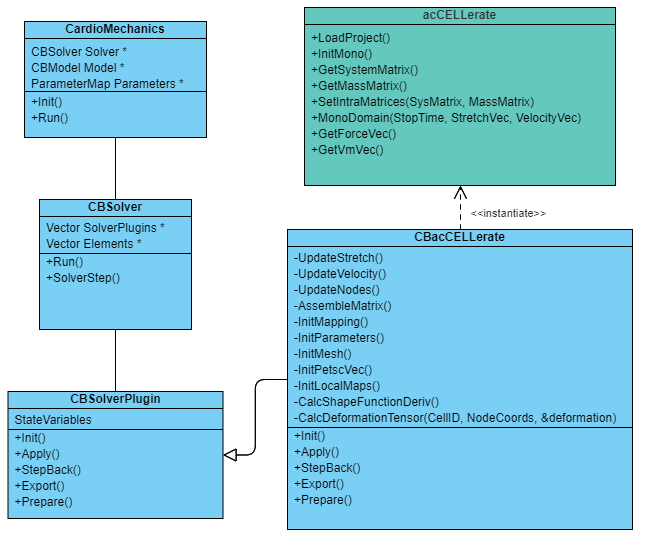
\includegraphics[width=1\linewidth]{Graphics/Classdiagram CBacCELLerate.png}
    \caption{Class diagram of the plugin CBacCELLerate, which acts as an interface to the electrophysiology solver acCELLerate.}
    \label{fig:CBacCELLerateUML}
\end{figure}

\paragraph{acCELLerate Specific Input Files} Since the plugin is only an interface to an entirely different software, we need to provide an extra set of input files that are specific to the electrophysiology simulator \ACC.
An overview can be found in \nameref{files:acCELLerate}.
The files that are required to run coupled simulations are the \nameref{files:ACCConfig}, \nameref{files:condition}, \nameref{files:material}, \nameref{files:cellmodel}, \nameref{files:ionmodel}, precalculated mass and stiffness matrices in PETSc format, and the mesh as a \nameref{subsubsec:VTK}.
Providing a mass and stiffness matrix is necessary for \ACC~to be initialized properly.
\CM~takes advantage of this by directly copying the parallel allocation of the matrices.
Both of these matrices can be set up using the tool \nameref{tools:BidomainMatrixGenerator}.

For efficiency reasons, the \verb|Export| option will interpolate $\Cai$ and transmembrane voltage $\u$ onto the mechanical mesh.\footnote{Exporting on the electrophysiology mesh slowed down the simulation significantly and increased storage requirements dramatically due to the high mesh resolution. If you use the native export of \ACC, it will still slow down the simulation and increase storage requirements but not as significantly, since it will export binary PETSc vectors instead of VTK.}
If high resolution data on the electrophysiology mesh is required, activate export in the \nameref{files:ACCConfig} or use a \nameref{files:Sensor} for specific point data.
With \verb|MEF| set to \verb|NONE|, deformation is ignored in the monodomain equation, \verb|FULL| will follow Algorithm \autoref{alg:CMEPCoupling}.
Using the option \verb|Material| defines the \textbf{mechanical} materials to be used for coupling.
It is important that these materials exist in both the mechanical and electrophysiological mesh (even though the material number does not need to be the same).
Ideally, the points of the EP mesh lie within the mechanical mesh elements or on the edges of them to ensure that the mapping algorithm works properly.
In general, mesh features that exist in the EP mesh should exist in the mechanics mesh as well.
This is not necessarily the case the other way around.
The \verb|INT| array specified using the option \verb|TissuePriority| defines a custom material priority list.
Materials with higher precedence should be given first.
This is especially important for smaller structures such as pectinate muscles or a thin endocardial layer that might only have a one element thickness.
In such a case, if the surrounding tissue would have a higher precedence, the smaller structure is not properly considered when building the matrices.
By default, lower numbers are prioritized, \ie 1, 2, 3, 4, ..., 255.
Make sure to use the same tissue priority list when you allocate the matrices with \nameref{tools:BidomainMatrixGenerator}.
Supply the \nameref{files:material} using the option \verb|MaterialFile| and the \nameref{files:ACCConfig} using the option \verb|ProjectFile|.
The mesh for electrophysiology should be given as a \nameref{subsubsec:VTK}
using the option \verb|acCELLerateMesh| and needs to contain the arrays \verb|Material|, \verb|Fiber|, \verb|Sheet|, and \verb|Sheetnormal|.

\begin{lstlisting}[language=XML,caption=.xml settings for the acCELLerate plugin]
<acCELLerate>
    <ProjectFile> STR </ProjectFile>
    <acCELLerateMesh> STR </acCELLerateMesh>
    <Permute> false </Permute>
    <MaterialFile> STR </MaterialFile>
    <TissuePriority> INT, INT, ... </TissuePriority>
    <ResultPreFix> STR </ResultPreFix>
    <ResultFolder> STR </ResultFolder>
    <PvdFileName> STR </PvdFileName>
    <Export> true </Export>
    <MEF> NONE/FULL </MEF>
    <Material> INT, INT, ... </Material>
    <OffsetTime> FLOAT </OffsetTime> <!-- [s] -->
    <constStretchRate> false </constStretchRate>
</acCELLerate>
\end{lstlisting}

\subsection{Export}
\label{subsec:Export}

Data export is defined in the \nameref{subsubsec:CardioMechanicsConfig} inside the Export tag.
Currently, only export as VTK files is available.
Data is written to nodes and elements respectively.
Some data is written to individual text files.
Refer to \autoref{tab:options} for information about what is exported.
Try to keep exported data to a minimum, since it can significantly impact simulation performance and increase file size.
Plugins call their own \verb+Export()+ function which is individually controlled in the respective plugin settings.


\begin{table}[h!]
    \centering
    \caption{Export option for CardioMechanics. $k$ indexes elements; $n$ indexes time.}
    \label{tab:options}
    \begin{tabular}{cccc}
    \toprule
       Option & File type & Location &  Data exported\\
       \midrule
       Active Stress & VTK & CellData &  $T_a$\\
       Fiber  & VTK & CellData & $\vec F \vec f_0$\\
       Sheet  & VTK & CellData & $\vec F \vec s_0$\\
       SheetNormal  & VTK & CellData & $\vec F \vec n_0$\\
       Jacobian  & VTK & CellData & $J = \det(\vec F)$\\
       TetgenBases  & VTK, .bases & CellData & $\norm{\vec F \vec f_0}$,$\norm{\vec F \vec s_0}$,$\norm{\vec F \vec n_0}$ at each quadr. point\\
       Deformation  & VTK & CellData  & $\vec C = \vec F^\mathrm{T}\vec F$\\
       DeformationEnergy & Textfile & Scalar & $E_\mathrm{def} = \sum_k V_0^k \Psi^k$\\
       ModelVolume & Textfile & Scalar & $V = \sum_k J^k/6$\\
       Lambda  & VTK & CellData  & $\sqrt{\vec F \vec f_0 \vdot \vec F \vec f_0}$, $\sqrt{\vec F \vec s_0 \vdot \vec F \vec s_0}$, $\sqrt{\vec F \vec n_0 \vdot \vec F \vec n_0}$ \\
       Cauchy & VTK & CellData  & $J^{-1} \vec F \vec S \vec F^\mathrm{T}$\\
       PK2Stress  & VTK & CellData & $\vec S$\\
       GreenLagrangeStrain & VTK & CellData & $E =0.5 (\vec C - \mathds{1})$\\
       LocalActivationTime & VTK & CellData  & $t_a$ (only when using an LAT file)\\
       KineticEnergy & Textfile & Scalar  & $E_\mathrm{kin} = 0.5 \vec M \vec v^2$\\
       DampingEnergyDissipation & Textfile & Scalar & $E_\mathrm{damp} = \sum_n \vec C_\mathrm{Rayleigh}^n \vec v^n \vec d^n$ \\
       TotalEnergy & Textfile & Scalar  & $E_\mathrm{tot} = E_\mathrm{damp} + E_\mathrm{def} + E_\mathrm{kin}$\\
       Displacement & VTK & PointData  & $\Delta \vec d^n$\\
       Velocity & VTK & PointData  & $\vec{\dot{d}}$\\
       Acceleration & VTK & PointData  & $\vec{\Ddot{d}}$\\
       AbsDisplacement & VTK & PointData  & $\sum^n_{0} \vec d^n$\\
       NodalForces & VTK & PointData  & $f_\mathrm{int}+f_\mathrm{ext}$\\
         \bottomrule
    \end{tabular}
\end{table}

\begin{lstlisting}[language=XML,caption=.xml settings for data export options.]
<Export>
    <Format>	VTK 	</Format>
    <Prefix> 	prefix	</Prefix>
    <TimeStep> 	FLOAT	</TimeStep>
    <Options>
    	<!-- Solver export options default settings -->
    	<ActiveStress> 			true 	</ActiveStress>
    	<Fiber> 				true 	</Fiber>
    	<Sheet>					true 	</Sheet>
    	<SheetNormal>			false	</SheetNormal>
    	<Jacobian>				false	</Jacobian>
    	<TetgenBases>			false	</TetgenBases>
        <Deformation>			false	</Deformation>
        <DeformationEnergy>		true	</DeformationEnergy>
        <ModelVolume>           true    </ModelVolume>
    	<Lambda>				true	</Lambda>
    	<Cauchy>				false	</Cauchy>
    	<PK2Stress>				true	</PK2Stress>
    	<GreenLagrangeStrain> 	true 	</GreenLagrangeStrain>
    	<LocalActivationTime>	false	</LocalActivationTime>
    	<!-- Newmark export options default settings -->
    	<KineticEnergy>				false	</KineticEnergy>
    	<DampingEnergyDissipation> 	false 	</DampingEnergyDissipation>
    	<TotalEnergy>				false	</TotalEnergy>
    	<Displacement>				true	</Displacement>
    	<Velocity>					true	</Velocity>
    	<Acceleration>				true	</Acceleration>
    	<AbsDisplacement>			true	</AbsDisplacement>
    	<NodalForces>				false	</NodalForces>
    </Options>
</Export>
\end{lstlisting}